% Generated from ../preprint.md by scripts/build_preprint.py.
% Generated manuscript template; scripts/build_preprint.py supplies the body.
\documentclass[11pt,a4paper]{article}
\usepackage[margin=25mm,headheight=14pt,headsep=7mm]{geometry}
\usepackage{amsmath,amssymb}
\usepackage{fontspec}
\usepackage{unicode-math}
\setmainfont{texgyretermes}[Extension=.otf,UprightFont=*-regular,
  BoldFont=*-bold,ItalicFont=*-italic,BoldItalicFont=*-bolditalic]
\setmathfont{texgyretermes-math.otf}
\setmonofont{texgyrecursor}[Extension=.otf,UprightFont=*-regular,
  BoldFont=*-bold,ItalicFont=*-italic,BoldItalicFont=*-bolditalic,Scale=0.82]
\usepackage{microtype}
\usepackage{setspace}
\setstretch{1.12}
\setlength{\parindent}{0pt}
\setlength{\parskip}{5pt plus 1pt minus 1pt}
\usepackage{graphicx,booktabs,array,longtable,calc}
\usepackage{caption}
\captionsetup{font={small,stretch=1.05},labelfont=bf,labelsep=period,
  justification=justified,singlelinecheck=false,skip=7pt}
\captionsetup[table]{position=above}
\renewcommand{\arraystretch}{1.22}
\setlength{\tabcolsep}{4pt}
\setlength{\textfloatsep}{14pt plus 2pt minus 2pt}
\setlength{\intextsep}{14pt plus 2pt minus 2pt}
\renewcommand{\topfraction}{0.92}
\renewcommand{\bottomfraction}{0.85}
\renewcommand{\textfraction}{0.08}
\renewcommand{\floatpagefraction}{0.72}
\makeatletter
\setlength{\@fptop}{0pt}
\makeatother
\usepackage[section]{placeins}
\usepackage{needspace}
\usepackage{titlesec}
\titleformat{\section}{\large\bfseries}{\thesection.}{0.55em}{}
\titleformat{\subsection}{\normalsize\bfseries}{\thesubsection}{0.65em}{}
\titlespacing*{\section}{0pt}{16pt plus 3pt minus 2pt}{7pt}
\titlespacing*{\subsection}{0pt}{12pt plus 2pt minus 2pt}{5pt}
\setcounter{secnumdepth}{2}
\usepackage{enumitem}
\setlist{topsep=5pt,itemsep=4pt,parsep=2pt,leftmargin=*}
\providecommand{\tightlist}{\setlength{\itemsep}{3pt}\setlength{\parskip}{0pt}}
\usepackage{fancyhdr}
\pagestyle{fancy}
\fancyhf{}
\fancyhead[L]{\footnotesize Cross-species transcriptomic comparisons}
\fancyhead[R]{\footnotesize Preprint}
\fancyfoot[C]{\thepage}
\renewcommand{\headrulewidth}{0.3pt}
\fancypagestyle{plain}{\fancyhf{}\fancyfoot[C]{\thepage}\renewcommand{\headrulewidth}{0pt}}
\usepackage{xcolor}
\definecolor{LinkBlue}{HTML}{174F70}
\usepackage{cite}
\usepackage{xurl}
\usepackage[colorlinks=true,allcolors=LinkBlue,bookmarksnumbered=true]{hyperref}
\usepackage{bookmark}
\hypersetup{pdftitle={Reliability and limits of cross-species
transcriptomic comparisons},pdfauthor={Zihui Zhang, Wei Wang, Ziyan
Zhou, Chen Peng, Zhi Wang},pdfcreator={Pandoc and LaTeX}}
\urlstyle{same}
% Mathematical Unicode in narrative text is explicitly mapped to the math font.
\usepackage{newunicodechar}
\newunicodechar{ρ}{\ensuremath{\rho}}
\newunicodechar{α}{\ensuremath{\alpha}}
\newunicodechar{β}{\ensuremath{\beta}}
\newunicodechar{Δ}{\ensuremath{\Delta}}
\newunicodechar{Σ}{\ensuremath{\Sigma}}
\newunicodechar{λ}{\ensuremath{\lambda}}
\newunicodechar{σ}{\ensuremath{\sigma}}
\newunicodechar{δ}{\ensuremath{\delta}}
\newunicodechar{√}{\ensuremath{\sqrt{\vphantom{x}}}}
\newunicodechar{≤}{\ensuremath{\leq}}
\newunicodechar{≥}{\ensuremath{\geq}}
\newunicodechar{→}{\ensuremath{\rightarrow}}
\newunicodechar{∞}{\ensuremath{\infty}}
\newunicodechar{×}{\ensuremath{\times}}
\newunicodechar{−}{\ensuremath{-}}
\newunicodechar{²}{\ensuremath{^{2}}}
\newunicodechar{₁}{\ensuremath{_{1}}}
\newunicodechar{₂}{\ensuremath{_{2}}}
\setlength{\emergencystretch}{2em}
\clubpenalty=10000
\widowpenalty=10000
\displaywidowpenalty=10000
\raggedbottom
\begin{document}
\thispagestyle{plain}
{\fontsize{19}{22}\selectfont\bfseries\raggedright Reliability and
limits of cross-species transcriptomic comparisons\par}
\vspace{7pt}
{\fontsize{11.5}{14}\selectfont \textbf{Zihui Zhang\textsuperscript{1},
Wei Wang\textsuperscript{2}, Ziyan Zhou\textsuperscript{2}, Chen
Peng\textsuperscript{1,*}, Zhi Wang\textsuperscript{2,*}}\par}
\vspace{4pt}
{\fontsize{9.5}{11.8}\selectfont\setstretch{1.05}\setlength{\parskip}{3pt}
\raggedright\hyphenpenalty=10000
\textsuperscript{1} National Key Laboratory of Veterinary Public Health,
College of Veterinary Medicine, China Agricultural University, Beijing,
China

\textsuperscript{2} Beijing Point Eight Intelligent Technology Co.,
Ltd., Beijing, China

\textbf{*Correspondence:} Chen Peng
(\href{mailto:pengchenea@cau.edu.cn}{\nolinkurl{pengchenea@cau.edu.cn}});
Zhi Wang
(\href{mailto:witwang@pointeight.ai}{\nolinkurl{witwang@pointeight.ai}}).

\textbf{Other author emails:} Zihui Zhang
(\href{mailto:18322383991@163.com}{\nolinkurl{18322383991@163.com}});\\
Wei Wang
(\href{mailto:mojie@pointeight.ai}{\nolinkurl{mojie@pointeight.ai}});
Ziyan Zhou
(\href{mailto:zy@pointeight.ai}{\nolinkurl{zy@pointeight.ai}}).
\par}
\vspace{5pt}
{\small Preprint --- version 2 --- 2026-10-26\par}
\vspace{11pt}
\pdfbookmark[1]{Abstract}{abstract}
\section*{Abstract}
\begingroup
\fontsize{10.5}{12.8}\selectfont

Whether a model organism anticipates human biology has been argued for a
decade from the same data, because the quantity that would settle it ---
how precisely the comparison itself is measured --- is almost never
reported. We measure it, and use it to price experimental choices
against one another.

Splitting subjects within each timepoint of a ten-species ex vivo blood
panel and recomputing the species-by-species redundancy matrix gives
split-half reliabilities averaging 0.900, 0.947 extrapolated to the full
subject set. A failure to transfer becomes a bounded statement rather
than an ambiguous one.

Dividing an observed agreement by what the data's own replicates permit
yields a quantity that cannot exceed one. It did, in three unrelated
datasets, every time because treated arms shared a control set; in the
largest, a quarter of all comparisons breached the bound, reaching 2.68.
The construction is therefore also a contamination test, and one that
needs no model, because it reads the design rather than the biology.

On that scale experimental choices become commensurable. With time and
dose matched, a rat-to-human hepatocyte comparison retains 15.2\% of its
ceiling; a threefold sampling-time mismatch within one species retains
32--45\%, a twelvefold 9--12\%. Paired on compound, the threefold
mismatch costs significantly less than the species change and, in rat,
the twelvefold costs more --- so aligning time, which is free, outranks
the choice of organism. Panels saturate early: the best two of six
livestock and rodent donors reach 77\% of the pool's asymptote and all
six reach 83\%, and because that asymptote is set by redundancy between
species rather than by effort, the curve a collection will follow can be
computed before it is commissioned.

Two results bound what the exchange rate can be used for. What crosses a
species boundary is mostly the response shared across perturbations (r =
0.333) rather than the part identifying one (r = 0.083); and a cultured
profile does not detectably predict organ injury in the animal, where
the in vivo profile does.

\endgroup
\clearpage

\section{Introduction}\label{introduction}

Whether a model organism anticipates human biology has been contested
for more than a decade with the same data supporting both answers. Seok
et al.~\cite{ref1} reported that murine orthologues matched their human
counterparts close to randomly in whole-blood leukocytes (R² between 0.0
and 0.1); Takao and Miyakawa \cite{ref2}, restricting to genes significant
in both species, reported Spearman correlations of 0.43--0.68 with
77--93\% agreement in direction; Shay et al.~\cite{ref3} recovered R =
0.38--0.45 and attributed the difference to time-frame alignment and to
the use of whole blood rather than purified cells. Hagai et al.~\cite{ref4}
found significant positive response correlation in every cross-species
pair of matched purified cells. The disagreement is not about the data.
It is about three methodological choices --- which genes enter, whether
sampling times are aligned, and what preparation is profiled --- none of
which is priced.

At the programme level the question has a long-standing empirical
answer. Olson et al.~\cite{ref5} reported true-positive concordance of 71\%
when rodent and non-rodent data were combined, 63\% for non-rodents
alone and 43\% for rodents alone; Monticello et al.~\cite{ref6} found the
non-human primate strongest over 182 blinded molecules; Atkins et
al.~\cite{ref7} reported median positive predictive values of 0.60 for
monkey against 0.41 for rat. The ordering is settled. What that
literature cannot supply is resolution --- a per-gene, per-context
quantity in which the cost of one experimental choice can be weighed
against another.

For a panel of species rather than a single pair, the object that
carries that resolution is not a number but a matrix: for a given
experimental context, the agreement between every pair of species'
perturbation responses. We write it ρ and call it the redundancy matrix,
because its entries say how much of what one species reports a second
species also reports. Matrices of this shape are reported throughout
comparative transcriptomics, and the same object under another name
organises representational analysis in systems neuroscience \cite{ref24}.
How precisely any particular one of them is measured is a different
question, and it is the one left open. Whether a dissimilarity measure
is reliable has been studied in its own right --- Walther et al.
\cite{ref32} compare classification accuracy, Euclidean and Mahalanobis
distance and correlation distance on exactly that criterion --- but that
is a choice between measures, made once for a field. The precision of
the matrix in hand, in the experiment that produced it, is essentially
never reported beside it. The field's current benchmark of
perturbation-response models, eleven methods over seven datasets,
reports neither a noise ceiling nor a reliability normalisation
\cite{ref61}. Without that number a comparison that comes back low cannot be
read: a failure to transfer and a failure to measure look the same.

A denominator for such a quantity is available. Correcting an observed
association by the geometric mean of the two measures' reliabilities
dates to Spearman \cite{ref8}; Archer et al.~\cite{ref9} applied exactly this
correction to cross-platform expression; systems neuroscience reports
model performance as CC\_norm, an observed correlation over a noise
ceiling estimated from repeats \cite{ref10,ref11}; and Zong et al.~\cite{ref12}
brought the construction to cross-species transcriptomics, reporting a
median congruence of 0.15 for human against mouse against 0.43 for human
against human. We adopt that denominator and use it for a purpose it has
not been put to: placing time, species and system on one scale so that
an exchange rate between them can be read off. Dose cannot be placed on
that scale in these data, for a reason that is itself a result (Section~\ref{ceiling-normalisation-and-the-exceeds-unity-bound}).

The measurements rest on five panels. An ex vivo whole-blood panel of
ten mammals under endotoxin carries the reliability, the species
ordering and every result about ρ, because it is the only one of the
five with enough subjects per species to split. Human and rat primary
hepatocytes and rat liver in vivo, from TG-GATEs, carry the boundary
pricing, because they are the only arms that hold time, dose and
compound fixed while changing one thing at a time. Three further panels
--- a five-species hepatocyte panel, bone-marrow-derived macrophages
from nine species, and seven yeasts --- test whether the saturation
result depends on the first panel. Section~\ref{methods} describes them and Section~\ref{data-and-code-availability} lists their accessions.

We report three things and bound their use. First, how precisely ρ is
measured, which is what makes the rest of the paper decidable. Second,
that expressing any agreement as a fraction of what its own replicates
permit yields a quantity that cannot exceed one, so an estimate above
one is a signal about the data rather than about biology; it fired twice
here, and both times the cause was the same. Third, an exchange rate
between a species change, a sampling-time mismatch and the step from
culture to animal, read on that common scale. Two negative results bound
what the exchange rate can be used for, and a standalone Limitations
subsection states what the design cannot settle.

\section{Results}\label{results}

Figure~\ref{fig:1} gives a standalone overview of the framework. Matched response
profiles enter two complementary calculations: species-pair redundancy
with subject-split reliability, and replicate-based ceilings for
comparisons across experimental boundaries. Figures 2--4 then report
donor value and panel saturation, context transfer, and response
specificity.

\begin{figure}[!htbp]
\centering
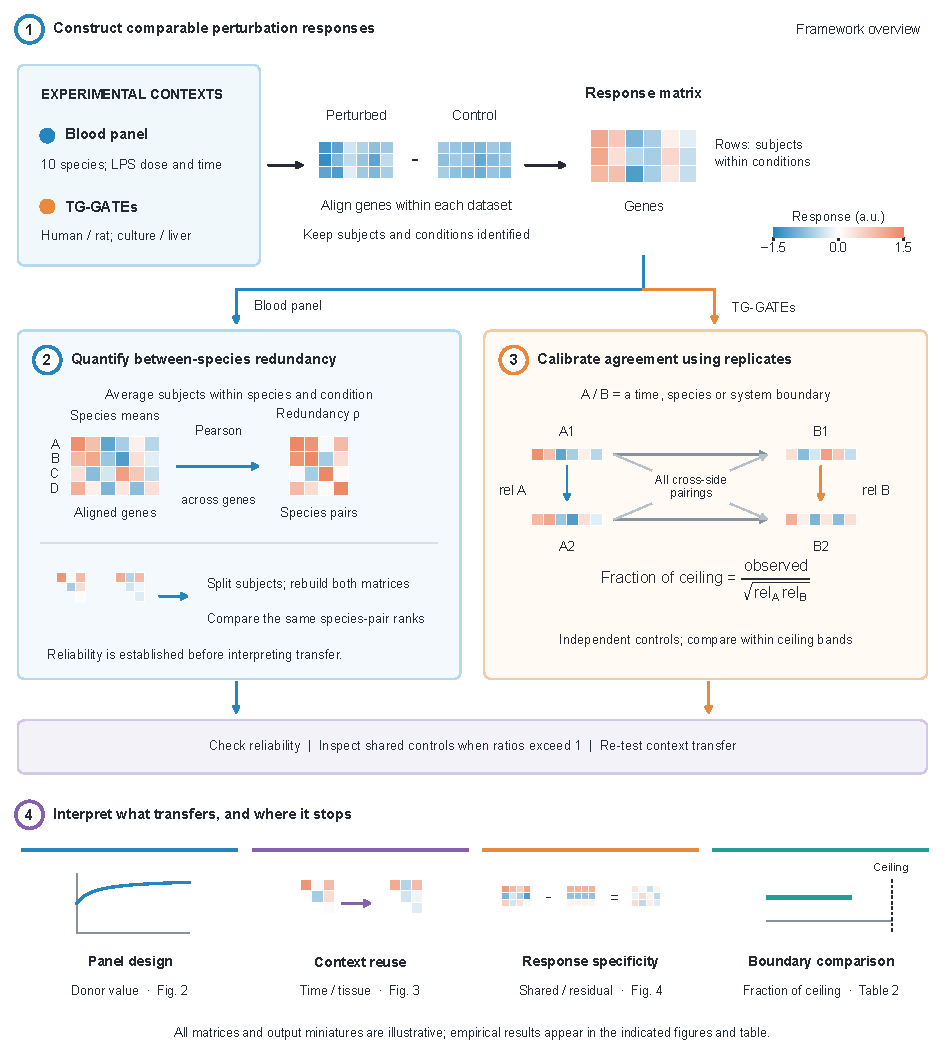
\includegraphics[width=\linewidth]{figures/Fig1.pdf}
\caption{Workflow for assessing cross-species transcriptomic agreement. \textbf{1}, Perturbation responses are constructed relative to controls on a common gene axis within each dataset, retaining subject and condition identities. The blood panel comprises ten species exposed to lipopolysaccharide (LPS); TG-GATEs provides human and rat hepatocytes and rat liver in vivo. \textbf{2}, For the blood panel, species-mean response profiles are correlated across genes to form the redundancy matrix, ρ. Subjects are split within each timepoint, both matrices are rebuilt, and the ranks of corresponding species pairs are compared to establish matrix reliability. \textbf{3}, For TG-GATEs boundary comparisons, within-side replicate response correlations, \(\mathrm{rel}_A\) and \(\mathrm{rel}_B\), define the ceiling; observed agreement averages cross-side replicate pairings. Control-disjoint contrasts are compared within ceiling bands. Ratios above one prompt inspection for sampling error or shared-control structure (Section~\ref{ceiling-normalisation-and-the-exceeds-unity-bound}). This profile-level ceiling and matrix reliability are different constructions. \textbf{4}, The framework supports panel design, tests of context reuse and response specificity, and comparisons of experimental boundaries. All displayed matrices and output miniatures are illustrative; they are not fitted or measured results. Blue-to-orange matrix colours denote negative-to-positive values; response matrices use arbitrary units, while correlation matrices span −1 to +1. Dataset-specific preprocessing and additional validation panels are described in Methods.}\label{fig:1}
\end{figure}

\subsection{Reliability of the redundancy
matrix}\label{reliability-of-the-redundancy-matrix}

Splitting the subjects within each timepoint of the blood panel and
computing ρ twice gives the split-half reliabilities of Table~\ref{tab:1}. They
average 0.900, which the Spearman-Brown extrapolation \cite{ref38,ref39} to
the full subject set raises to 0.947. The 2 h matrix is the least
precisely measured of the three on every reading, so the comparisons
that rest on it are the weakest.

\begin{table}[!htbp]
\centering
\small
\caption{Split-half reliability of ρ: the matrix computed from one half of the subjects against the matrix computed from the other, within a timepoint. Spearman over species pairs. 45 pairs over ten species, 35 of them spanning different taxonomic orders; the partial removes a graded taxonomic distance from both sides.}\label{tab:1}
\begin{tabular}{@{}>{\raggedright\arraybackslash}p{(\linewidth - 6\tabcolsep) * \real{0.16}}
>{\centering\arraybackslash}p{(\linewidth - 6\tabcolsep) * \real{0.23}}
>{\centering\arraybackslash}p{(\linewidth - 6\tabcolsep) * \real{0.27}}
>{\centering\arraybackslash}p{(\linewidth - 6\tabcolsep) * \real{0.34}}@{}}
\toprule
\textbf{Timepoint} & \textbf{All 45 pairs} & \textbf{35 cross-order pairs} & \textbf{Partial on taxonomic distance} \\
\midrule
2 h & 0.817 & 0.670 & 0.738 \\
\addlinespace[3pt]
6 h & 0.955 & 0.926 & 0.945 \\
\addlinespace[3pt]
24 h & 0.928 & 0.901 & 0.922 \\
\bottomrule
\end{tabular}
\end{table}

That number is what makes the blood panel's results decidable. Where ρ
transfers there, the transfer is not an artefact of noise; where it does
not, the failure cannot be blamed on imprecision either. Both directions
are used below, and the second is the one that is usually unavailable.
It does not extend to the comparison panels, which carry one sample per
species and so support no reliability of their own --- the cross-tissue
nulls of Section~\ref{reuse-of-the-matrix-across-contexts} are undecidable for exactly that reason.

\subsection{Ceiling normalisation and the exceeds-unity
bound}\label{ceiling-normalisation-and-the-exceeds-unity-bound}

Figure~\ref{fig:2}a fixes the correlation unit that Sections 2.3, 2.5, 3.1 and 3.2
read values in: for each donor species, the agreement between its
response and the held-out human response in the blood panel. The scale
this section builds is the second one, and it is what Table~\ref{tab:2} below
uses.

The reliability in Section~\ref{reliability-of-the-redundancy-matrix} is a special case of a construction that
applies to any comparison; Svensson et al.~\cite{ref62} score
perturbation-response models against a half-sample reference ceiling of
the same family. Here it is applied to experimental boundaries rather
than to models, and built on donors rather than cells, because a cell
split approaches unity as sequencing depth rises and leaves no asymptote
below one to read. For each perturbation we compute the correlation
between two sides across genes, and divide it by the same statistic
computed between replicates within each side:

\[\text{fraction of ceiling} = \frac{\text{observed}}{\sqrt{\mathrm{rel}_A\,\mathrm{rel}_B}}\]

The population quantity cannot exceed unity, so an estimate above it is
either sampling error in the two replicate correlations or structure
shared between the two sides before any biology, and the quantity
doubles as a diagnostic. That a shared reference can manufacture
correlation between arms that have none is a known failure mode of
normalisation \cite{ref54}, and it is the one these data turned out to have.
It fired on the dose contrasts in two unrelated datasets and, in both,
the mechanism was confirmed directly: the dose arms at one timepoint are
referenced to a shared control set (one experiment identifier covering
all four arms in 145/145 and 143/143 compounds). Between two and
thirty-eight compounds per dose contrast exceed the bound, to a maximum
of 1.97. Those contrasts are excluded throughout.

A third dataset was brought in to test the construction rather than to
be analysed, and there the breach is not marginal. In LINCS L1000 Phase
2, 948 plates each carry a median of 20 control wells against 350
treated, so every treated well on a plate is referenced to the same
small control set. Predicting one cell line's response from another's
over 1,785 compounds, 471 of the 1,912 units for which a ceiling can be
formed exceed it --- a quarter of them --- reaching 2.68 against a bound
of one. The geometry that produces this is visible in the plate layout
before any statistic is computed, which is the case for the diagnostic:
it detects a property of the design, not of the biology, and it needs no
model to do so.

Because the fraction of ceiling tracks its own denominator (Spearman
+0.665 against the ceiling, +0.544 against response amplitude, n = 123),
rows are compared only inside a fixed ceiling band.

\begin{table}[!htbp]
\centering
\small
\caption{Fraction of ceiling retained, read from compounds whose ceiling falls in the band {[}0.60, 0.78). TG-GATEs human and rat primary hepatocytes and rat liver in vivo; gene-level Pearson; median over compounds, both columns read inside the band. The shuffle-corrected column subtracts what a randomly paired compound yields.}\label{tab:2}
\begin{tabular}{@{}>{\raggedright\arraybackslash}p{(\linewidth - 6\tabcolsep) * \real{0.53}}
>{\centering\arraybackslash}p{(\linewidth - 6\tabcolsep) * \real{0.16}}
>{\centering\arraybackslash}p{(\linewidth - 6\tabcolsep) * \real{0.23}}
>{\centering\arraybackslash}p{(\linewidth - 6\tabcolsep) * \real{0.08}}@{}}
\toprule
\textbf{Change} & \textbf{\% of ceiling} & \textbf{Shuffle-corrected} & \textbf{n} \\
\midrule
rat liver in vivo, 24 h vs 9 h & 52.6 & 36.5 & 38 \\
\addlinespace[3pt]
rat liver, single 24 h vs repeat 4 d & 51.6 & 35.2 & 36 \\
\addlinespace[3pt]
human hepatocyte, 24 h vs 8 h & 44.8 & --- & 41 \\
\addlinespace[3pt]
rat liver in vivo, 24 h vs 6 h & 42.2 & 27.0 & 43 \\
\addlinespace[3pt]
rat hepatocyte, 24 h vs 8 h & 32.0 & --- & 34 \\
\addlinespace[3pt]
rat liver in vivo, 24 h vs 3 h & 25.6 & 13.0 & 37 \\
\addlinespace[3pt]
\textbf{species, human vs rat hepatocyte} & \textbf{15.2} & \textbf{7.5} & 38 \\
\addlinespace[3pt]
human hepatocyte, 24 h vs 2 h & 12.4 & --- & 20 \\
\addlinespace[3pt]
rat hepatocyte, 24 h vs 2 h & 9.0 & --- & 53 \\
\addlinespace[3pt]
\textbf{system, dish vs animal (time matched)} & \textbf{8.6} & \textbf{1.6} & 61 \\
\addlinespace[3pt]
species and system together & 3.5 & 0.8 & 51 \\
\bottomrule
\end{tabular}
\end{table}

A threefold mismatch in sampling time costs less than a species change;
a twelvefold mismatch costs more. Because the table's rows are medians
over partly disjoint compound sets, we test that ordering on compounds
measured on both sides. Pairing on compound, the threefold mismatch
retains 20.5 percentage points more of its ceiling than the species
change in rat hepatocytes (114 of 129 compounds, sign test p = 5 ×
\ensuremath{10^{-20}}) and 24.2 points more in human (124 of 129, p = 8 × \ensuremath{10^{-31}});
restricted to compounds inside the band on both sides the same contrasts
give +17.3 (16 of 19, p = 0.004) and +23.3 (18 of 18, p = 8 × \ensuremath{10^{-6}}). The
twelvefold mismatch reverses: in rat it retains 7.7 points less than the
species change (35 of 129, p = 2 × \ensuremath{10^{-7}}; in band −8.5, 3 of 15, p =
0.035), and in human the 47 shared compounds give −2.3 points and do not
resolve it (p = 0.24). The system row is the one that needed the
single-dose in vivo arm, sampled at 3, 6, 9 and 24 hours, to overlap the
in vitro grid. Read as medians it sits below the species row, 8.6\%
against 15.2\%. \textbf{That ordering does not survive the test we have
just applied to the others.} On the sixteen compounds measured inside
the band on both sides, the paired difference is +0.8 points with 8 of
16 favouring the system change, sign test p = 1.00. We therefore report
the two medians and state that the dish-to-animal step and the species
step do not separate in these data, rather than ordering them.

\subsection{Saturation with panel
size}\label{saturation-with-panel-size}

\begin{figure}[!htbp]
\centering
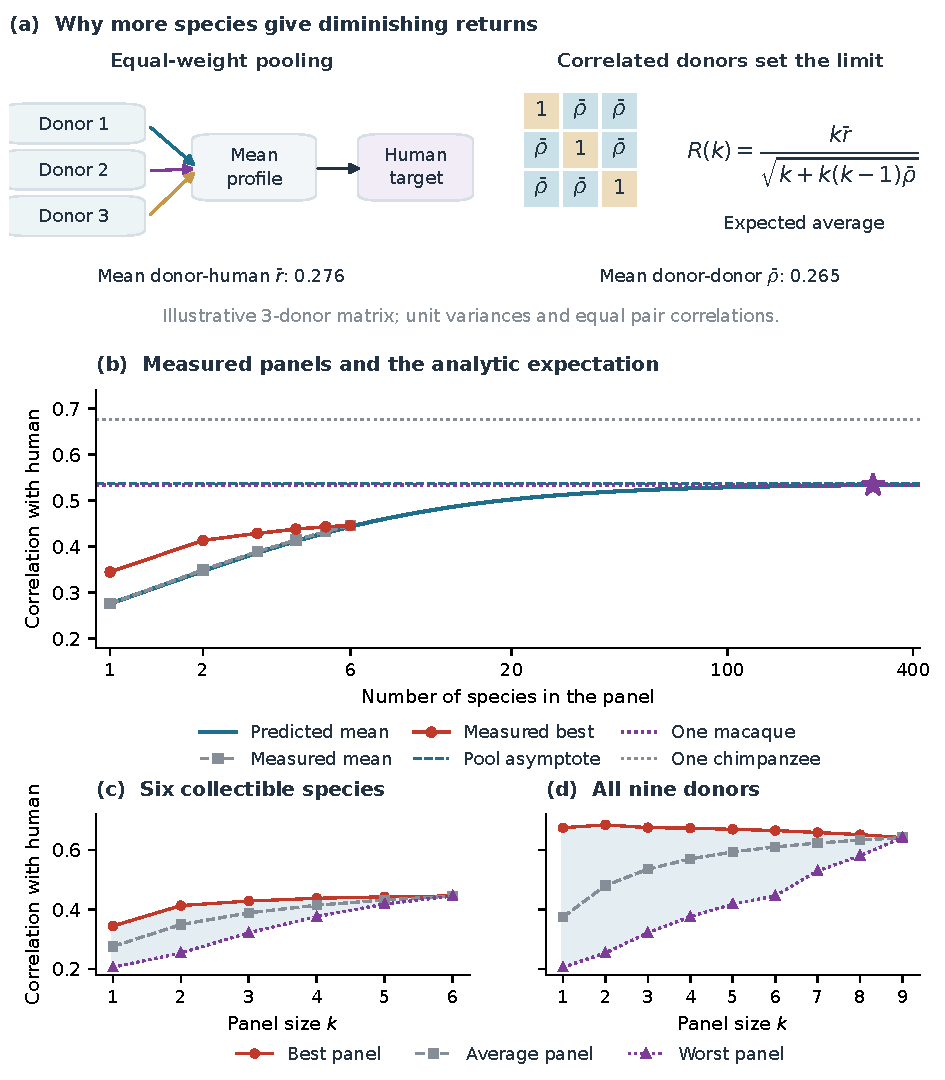
\includegraphics[width=\linewidth]{figures/Fig2.pdf}
\caption{Donor value, panel composition and the limits of pooling. \textbf{(a)} Mean across-gene Pearson correlation between each donor species and the held-out human response, over nine endotoxin conditions in ex vivo blood (25,638 genes). Points and horizontal bars show estimates and 95\% stratified leave-one-subject-out jackknife intervals. Absolute values are low by 0.022 to 0.062 under the missing-value convention of Section~\ref{limitations}. \textbf{(b, c)} Best (orange circles), mean (blue squares) and worst (grey triangles) equal-weight subsets at each size, enumerated among the six non-primate donors and all nine donors, respectively. Shading is the full range across subsets, not an uncertainty interval; both panels share the same vertical scale. \textbf{(d)} The exchangeable-predictor expectation R(k), using measured mean donor--human \ensuremath{\bar{r}} = 0.276 and donor--donor \ensuremath{\bar{\rho}} = 0.265 for the six non-primate species, assumes unit variances and equal pair correlations. Blue squares are measured subset means. The grey region and dashed curve mark extrapolation beyond the six available donors. Horizontal references show the pool asymptote (0.536), one macaque (0.534) and one chimpanzee (0.676). The diamond marks the analytic crossing at k = 297, not a measured panel; this crossing disappears on the filtered gene axes of Section~\ref{controls-on-the-species-ordering}. All empirical panels use the same nine conditions and gene axis.}\label{fig:2}
\end{figure}

What a new species adds depends on how much of its response the species
already in the panel carry, so the saturation curve (Figure~\ref{fig:2}) is a
consequence of the matrix measured in Section~\ref{reliability-of-the-redundancy-matrix}.

Increments to the best panel are +0.069, +0.015, +0.009, +0.005 and
+0.003: the first step falls 4.5-fold and each step after that roughly
halves. In the full nine-donor pool the best panel peaks at two species
and declines monotonically thereafter. The saturation result does not
rest on this panel alone: it replicates in four further panels, two of
which --- the FAANG macrophages and the yeasts --- contain neither
primates nor human. The other two do, so that part of the replication is
not independent of the primate contrast.

For a homogeneous pool the measured curve follows the equal-weight form
for k exchangeable predictors,

\[R(k) = \frac{k\bar{r}}{\sqrt{k + k(k-1)\bar{\rho}}},
\qquad \lim_{k\to\infty} R(k) = \frac{\bar{r}}{\sqrt{\bar{\rho}}},\]

where \ensuremath{\bar{r}} is the mean correlation between a donor species and the human
target and \ensuremath{\bar{\rho}} the mean off-diagonal entry of ρ. The form is an
expectation over panels of size k and therefore describes the average
panel, not the best one. The form itself is classical: Kelley \cite{ref29}
gives it as the correlation between a criterion and an equally weighted
sum of k scores, with the two parameters entering as the mean
score-criterion and mean inter-score correlations, and takes the same k
→ ∞ limit; Gulliksen \cite{ref30} states that limit as a decision rule for
whether lengthening a test can raise its validity. Kelley reads it as
the correlation between the criterion and the true score the components
share, which is the one-sided correction for attenuation --- so the
asymptote here and the ceiling of Section~\ref{ceiling-normalisation-and-the-exceeds-unity-bound} are one construction seen
twice. An accuracy equation of the same shape is used to combine sources
in genomic prediction \cite{ref31}, there for two sources and with no
ceiling set by the correlation between them. This section adds the
measurement rather than the form: \ensuremath{\bar{\rho}} estimated for cross-species
perturbation responses, carrying the reliability of Section~\ref{reliability-of-the-redundancy-matrix}. Fitted
against the average panel it gives a residual sum of squares of 3.0 ×
\ensuremath{10^{-5}} over six points at \ensuremath{\bar{r}} = 0.276 and \ensuremath{\bar{\rho}} = 0.265; scored instead against
the best panel of each size --- a quantity it does not claim --- the
same fit returns 1.2 × \ensuremath{10^{-2}}, which is worse than a horizontal line (7.3
× \ensuremath{10^{-3}}). The asymptote is 0.536, with a leave-one-subject-out standard
error of 0.021. A single chimpanzee reaches 0.676, above that asymptote,
so no equal-weighted panel drawn from this pool reaches its level at any
size. A single macaque reaches 0.534, within one standard error of the
asymptote, so these data do not place it on either side: the gap is
+0.0025 with a paired interval of {[}−0.034, +0.039{]}. The six species
together reach 0.446, 83\% of their own asymptote, and adding all six to
one macaque buys +0.0086.

The fit degrades sharply on a heterogeneous pool: including a chimpanzee
raises the residual sum of squares against the average panel from 3.0 ×
\ensuremath{10^{-5}} to 5.5 × \ensuremath{10^{-3}} over nine points, a factor of 186. This is expected,
since exchangeability is the form's premise.

Panel size does buy insurance (Figure~\ref{fig:2}b, c), though the two readings
below come from different pools and the narrowing is not monotone in
either. In the nine-donor pool the spread between the best and the worst
panel of a given size narrows from 0.431 at k = 2 to 0.071 at k = 8. In
the six collectible species it is non-monotone, rising from 0.139 at k =
1 before falling, so the guarantee rather than the spread is the usable
statement: in an unfamiliar context, where the best donor is unknown, a
single-species choice ranges from 0.345 to 0.206 depending on the guess,
while the full six-species panel reached 0.446, the one value it can
take in this pool.

\subsection{Reuse of the matrix across
contexts}\label{reuse-of-the-matrix-across-contexts}

\begin{figure}[!htbp]
\centering
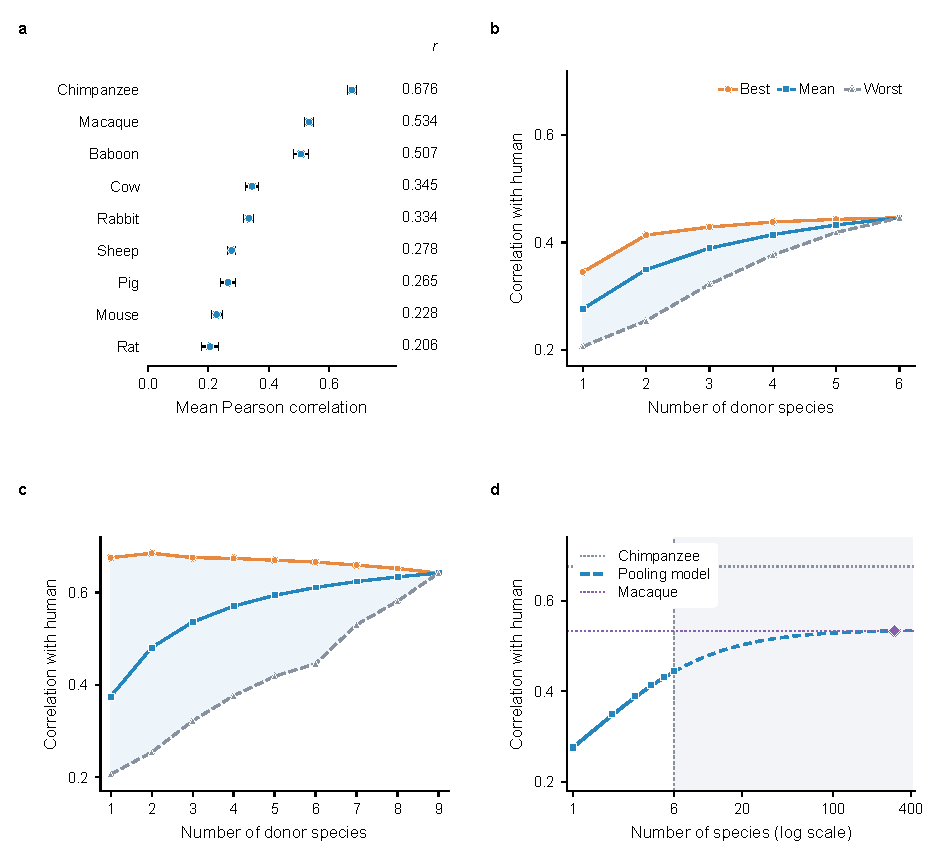
\includegraphics[width=\linewidth]{figures/Fig3.pdf}
\caption{Matrix reliability and transfer across contexts. \textbf{(a)} Illustrative upper-triangle matrices, matched-pair vectors and a rank plot show how matrix agreement is computed. Self-correlations and duplicate pairs are omitted. Purple outlines identify pair A--C; the rank plot's diagonal denotes equal ranks. \textbf{(b)} Measured split-half reliability within each blood timepoint. \textbf{(c)} Measured agreement between blood timepoints. Numbers and heatmap colours encode Spearman coefficients; the three columns use all pairs, cross-order pairs, and partial correlation after removing ranked taxonomic distance. Panels (b) and (c) use 45 species pairs, including 35 cross-order pairs. \textbf{(d)} Blood--macrophage agreement over ten shared pairs, six cross-order, shown for both estimators: pooling profiles before correlation, or correlating within conditions and then averaging. Grey circles, blue squares and purple diamonds correspond to the three analyses in (b, c). All empirical panels use the current two-estimator analysis. Asterisks mark nominal one-sided p \textless{} 0.05 under species-label Mantel permutations, without multiplicity adjustment. Neither cross-order blood--macrophage estimate is significant. The blood--hepatocyte comparison is reported in the text; its four cross-order pairs fall below the Methods floor of five.}\label{fig:3}
\end{figure}

Because the entire saturation curve is a function of ρ, the redundancy
matrix is the object worth transferring. Raw matrix agreement is
supported between neighbouring blood timepoints; the largest time gap
lacks support after taxonomic controls, and cross-tissue transfer
remains unestablished. The blood--macrophage comparison (Figure~\ref{fig:3}d)
depends on which of two estimators is used, and their cross-order signs
disagree, so we report both. Pooling conditions before computing ρ gives
Spearman +0.333 between blood and macrophage over all ten shared pairs
(Mantel p = 0.203); computing ρ inside each condition and averaging
gives +0.503 (p = 0.035). Under the cross-order restriction the two part
company: +0.371 for the per-condition estimator and −0.086 for the
pooled one, neither significant. The blood--hepatocyte comparison
reaches +0.60 over six pairs but at p = 0.337, so it does not support a
transfer claim before any restriction is applied. The absolute level
also shifts between contexts (mean 0.343, 0.420 and 0.307), so each
context requires its own measurement in any case. We draw no positive
cross-tissue conclusion from these numbers.

An ordering of species pairs invites the objection that it restates a
phylogeny, and the objection has to be answered with pairs whose
relatedness is matched. The objection has weight: taxonomic relatedness
is the basis of a deployed regulatory tool, the US EPA's interspecies
correlation estimation models, built from 780 models over 77 aquatic
species and more than 550 chemicals, in which same-family surrogates
predict within fivefold of the measured value 91\% of the time \cite{ref41}.
It also has a counterweight from the same field: across 36 datasets,
Coleman and Edmands \cite{ref42} found a strong phylogenetic signal in only
9, with no attribute shared by those nine. Neither study measures what
we measure --- both read a single acute endpoint in aquatic animals,
where this paper reads a transcriptome-wide response in mammals --- so
they bound how far the objection generalises rather than settling it.
The blood panel can supply them. Its preparation subtracts a no-LPS
control matched to each subject and timepoint, so the three timepoints
are control-disjoint and serve as three contexts across all ten species:
45 pairs, 35 of them spanning different taxonomic orders. Restricted to
those 35, and again with a graded taxonomic distance partialled out of
both sides, two of the three comparisons survive a Mantel null (Figure~\ref{fig:3}c, Table~\ref{tab:3}). The third survives neither: 2 h against 24 h falls to
+0.084 restricted and +0.262 partialled, at p = 0.374 and 0.122.

About half of this matrix is not pair-specific at all. Writing each
entry as a per-species level plus a pair interaction, the additive part
accounts for 44.5\%, 47.1\% and 56.2\% of the off-diagonal variance at
2, 6 and 24 hours. Removing it by double-centring and repeating the
three comparisons, all three now pass under the cross-order restriction,
and pass again with the graded taxonomic distance partialled out of both
sides, so the three do not pass merely because double-centring removed
the part that carries relatedness. Table~\ref{tab:3} gives both matrices side by
side.

The reason is not that the additive part fails to transfer. Measured
directly it transfers rather well, at Spearman +0.855, +0.600 and +0.794
across the three timepoint pairs, which is better than the interaction
manages. The mixture is what changes: the additive share rises from
44.5\% to 56.2\% and the spread of the per-species levels nearly
doubles, because by 24 hours the two rodents have fallen away from
everything else --- mouse from 0.401 to 0.072 and rat from 0.361 to
0.121, where the chimpanzee moves only from 0.461 to 0.310. When two
components are summed and their relative weight shifts between contexts,
the sum reproduces itself across contexts less well than either
component does on its own. Double-centring removes that shift in weight;
it does not remove a defect.

This buys a narrower and firmer statement than the raw matrix supports.
The pair-specific structure --- which is the object a catalogue would
sell, since the per-species level is one number and the structure is the
matrix --- reuses across all three contexts here, including the change
of regime. The per-species level also reuses, but its scale does not, so
the two should be carried separately rather than as one matrix.

\begin{table}[!htbp]
\centering
\small
\caption{Agreement between timepoint redundancy matrices before and after double-centring. Spearman over species pairs with a one-sided Mantel p beneath; 45 pairs, 35 cross-order. Raw rows use \protect\path{rho_cross_panel_both_estimators.json}, as in Figure~\ref{fig:3}; double-centred rows use \protect\path{rho_double_centred.json}. Both use average ranks for tied taxonomic distances. Each row's p-values come from its own permutation run. Minimum attainable Monte Carlo p-values are rounded to 5 × \ensuremath{10^{-5}} or 2.5 × \ensuremath{10^{-4}}; they indicate simulation resolution.}\label{tab:3}
\begin{tabular}{@{}>{\raggedright\arraybackslash}p{(\linewidth - 8\tabcolsep) * \real{0.15}}
>{\centering\arraybackslash}p{(\linewidth - 8\tabcolsep) * \real{0.16}}
>{\centering\arraybackslash}p{(\linewidth - 8\tabcolsep) * \real{0.23}}
>{\centering\arraybackslash}p{(\linewidth - 8\tabcolsep) * \real{0.23}}
>{\centering\arraybackslash}p{(\linewidth - 8\tabcolsep) * \real{0.23}}@{}}
\toprule
\textbf{Matrix} & \textbf{Comparison} & \textbf{All 45 pairs} & \textbf{35 cross-order} & \textbf{Partial on taxonomy} \\
\midrule
raw & 2 h vs 6 h & +0.684\newline (p = 5 × \ensuremath{10^{-5}}) & +0.515\newline (p = 0.020) & +0.581\newline (p = 0.0022) \\
\addlinespace[3pt]
raw & 2 h vs 24 h & +0.438\newline (p = 0.028) & +0.084\newline (p = 0.374) & +0.262\newline (p = 0.122) \\
\addlinespace[3pt]
raw & 6 h vs 24 h & +0.848\newline (p = 1 × \ensuremath{10^{-4}}) & +0.707\newline (p = 0.014) & +0.813\newline (p = 0.0012) \\
\addlinespace[3pt]
double-centred & 2 h vs 6 h & +0.878\newline (p = 5 × \ensuremath{10^{-5}}) & +0.749\newline (p = 1 × \ensuremath{10^{-4}}) & +0.849\newline (p = 2.5 × \ensuremath{10^{-4}}) \\
\addlinespace[3pt]
double-centred & 2 h vs 24 h & +0.717\newline (p = 5 × \ensuremath{10^{-5}}) & +0.417\newline (p = 0.009) & +0.643\newline (p = 2.5 × \ensuremath{10^{-4}}) \\
\addlinespace[3pt]
double-centred & 6 h vs 24 h & +0.879\newline (p = 5 × \ensuremath{10^{-5}}) & +0.755\newline (p = 5 × \ensuremath{10^{-5}}) & +0.851\newline (p = 2.5 × \ensuremath{10^{-4}}) \\
\bottomrule
\end{tabular}
\end{table}

The comparison that fails on the raw matrix is the one that spans the
largest gap, and it fails for a reason we had already measured elsewhere
in these data. Agreement does not decay smoothly with elapsed time: 6 h
against 24 h, a fourfold gap, retains more than 2 h against 6 h, a
threefold gap. The early timepoint behaves as a regime of its own, which
the TG-GATEs hepatocyte series shows independently --- 24 h against 8 h
retains 45\% of ceiling and 24 h against 2 h only 12\%. These data
therefore establish something narrower than reuse across contexts in
general. Raw matrix agreement is supported between neighbouring blood
timepoints, but not across the largest time gap after taxonomic
controls; its pair-specific part retains agreement across all three.

The same restriction applied across panels leaves six and four
cross-order pairs, and nothing survives it under either estimator. For
blood against macrophage the per-condition estimator gives +0.371
restricted and +0.103 partialled, the pooled one −0.086 and −0.313, none
significant; the blood--hepatocyte comparison retains four cross-order
pairs, too few for a correlation we report, and computed on exactly
those four it returns −0.400 (p = 0.788). Both comparison panels carry
one sample per species and so admit no reliability estimate of their
own. A failure to transfer therefore cannot be separated from a failure
to measure. The within-panel result establishes reusability within a
context family; reusability across tissues remains open, and the
measurement that would settle it needs donor replication in a new
comparison panel rather than more species.

\subsection{Controls on the species
ordering}\label{controls-on-the-species-ordering}

Two alternative explanations predict the same ordering as biology does,
and both were tested on the data in hand. The first is annotation
quality. A species whose genome is annotated less well maps fewer genes
onto the shared human axis; the unmapped positions enter as zeros, so
its log fold changes compress toward zero and correlate less with
anything. Because annotation quality tracks how much a species has been
studied, it also tracks relatedness to human, and so predicts the same
ordering biology does. Restricting to genes detectably expressed at rest
in all ten species removes that channel by construction. At thresholds
retaining 6,477, 5,372 and 2,973 genes the ordering is unchanged
(Spearman +0.98, +0.97 and +0.98 against the full-axis ranking) and
every value rises, chimpanzee from 0.676 to 0.857 and rat from 0.206 to
0.357. Annotation does carry part of the premium --- the primate to
non-primate ratio falls from 2.07 to 1.66 --- but it does not carry the
ordering.

The second is measurement precision, since a species with a small
response relative to noise correlates poorly with anything. The raw
ordering does track response amplitude at Spearman +0.93, which is why
the test is needed. Dividing by each species' own split-half
reliability, the normalisation this paper applies everywhere else,
leaves the ordering intact at Spearman +0.967; mouse and rat
reliabilities are 0.81 and 0.78, mid-pack among the nine, so their
position is not an artefact of measurement.

Figure~\ref{fig:2}a carries stratified leave-one-subject-out intervals, standard
errors 0.007 to 0.014. Overlap between two intervals is not a test, so
the ordering was checked by a paired jackknife on the difference, which
separates 33 of the 36 species pairs: cow against rabbit, sheep against
pig and mouse against rat do not separate. The tiers are resolved and
the ordering inside a tier is not.

The same gene sets were carried to the saturation curve, since the
pricing argument rests on a gap of 0.0025 between the asymptote and one
macaque while filtering moves every correlation by about 0.15. Both
parameters move together: \ensuremath{\bar{r}} rises from 0.276 to 0.408, 0.428 and 0.454
while \ensuremath{\bar{\rho}} rises from 0.265 to 0.391, 0.408 and 0.429, so the asymptote
rises more slowly than the macaque's level does and the gap goes from
+0.0025 to −0.0257, −0.0162 and −0.0092. On every filtered set the
collectible pool's ceiling sits below one macaque rather than above it,
and a paired jackknife over 36 subjects separates only the first:
−0.0257 {[}−0.050, −0.001{]}, −0.0162 {[}−0.041, +0.008{]} and −0.0092
{[}−0.031, +0.013{]}, against +0.0025 {[}−0.034, +0.039{]} on the
unfiltered axis. That conclusion rests on the filtered axes alone. On
the unfiltered axis, where the quantity was first computed, the gap has
the opposite sign, and Section~\ref{saturation-with-panel-size} declines to place the macaque on
either side. As the filter tightens, the margin shrinks monotonically,
and still does after normalising by the headroom each gene set leaves
(−8.0\%, −5.2\%, −3.1\%). Tighter filters leave fewer genes and widen
intervals, which explains the interval width but not the drift of the
point estimate toward zero, for which we have no explanation.

\subsection{Consensus and perturbation-specific
components}\label{consensus-and-perturbation-specific-components}

\begin{figure}[!htbp]
\centering
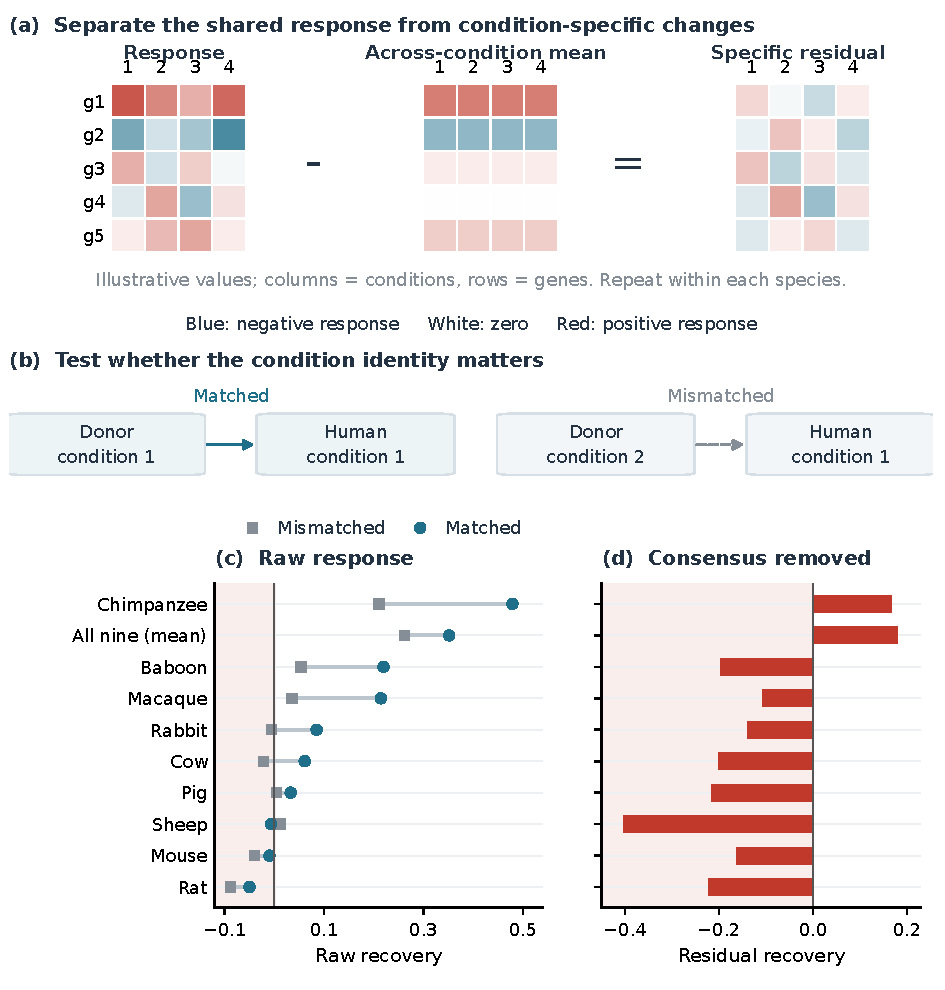
\includegraphics[width=\linewidth]{figures/Fig4.pdf}
\caption{Separating common and condition-specific responses in the blood panel. \textbf{(a)} Illustrative gene-by-condition matrices: subtract each species' across-condition mean from every condition to obtain its residual. All three matrices use the same scale, from −2 (blue) to +2 (orange), in arbitrary units. \textbf{(b)} An illustrative pairing map distinguishes matched donor--human conditions (blue diagonal) from mismatched conditions (grey off-diagonal). Four conditions are shown schematically; the empirical analysis uses nine. \textbf{(c)} Measured matched recovery (blue circles; mean over conditions) and mismatched recovery (grey squares; median over different-condition pairings), connected within each donor row. Segments compare scores and do not indicate uncertainty. \textbf{(d)} Recovery after mean subtraction on both sides, with rows aligned to (c); orange circles denote positive estimates and grey squares negative estimates, without implying significance. Stems connect each estimate to zero. Recovery is 1 − SSE/Σy²: zero is the no-response prediction and negative values are worse than that baseline. The statistic is unbounded below; the residual target changes the denominator, so magnitudes in (c) and (d) are not comparable. Only the chimpanzee and the nine-species equal-weight mean retain positive residual recovery.}\label{fig:4}
\end{figure}

What crosses a species boundary is mostly the response shared across
perturbations rather than the part that identifies one. Splitting a
perturbation profile into a shared component and a compound-specific
residual is not new: Szalai et al.~\cite{ref51} show that signatures of cell
death and proliferation dominate perturbation transcriptomics generally,
and frameworks for evaluating perturbation-response models now separate
the shared from the specific as a matter of course \cite{ref52}. What is new
here is the quantity, measured across a species boundary and against a
shuffled control. We decompose each profile into its projection on the
across-compound consensus and the residual. In TG-GATEs hepatocytes the
consensus transfers between species at r = 0.333 and the
compound-specific residual at r = 0.083. Pairing a compound's human
profile against a different compound's rat profile recovers 43\% of the
matched agreement. At the dish-to-animal boundary even less of the
agreement is compound-specific: 87\% of it survives shuffling the
compound pairing. Both percentages are taken over all shared compounds,
where Table~\ref{tab:2}'s two columns are in-band medians, so the two are not the
same ratio and should not be differenced.

The blood panel uses a direct subtraction of each species'
across-condition mean (Figure~\ref{fig:4}a), giving the pattern in Figure~\ref{fig:4}d. As
its caption explains, the sign is interpretable, while raw and residual
recovery magnitudes are not comparable. After the across-condition
consensus is removed, only the chimpanzee and the nine-species mean
remain positive.

\subsection{Prediction of organ injury from cultured and in vivo
profiles}\label{prediction-of-organ-injury-from-cultured-and-in-vivo-profiles}

With serum alanine and aspartate aminotransferase from the same rats
whose livers were profiled, a leave-one-compound-out similarity
predictor was run at every combination of three endpoints --- ALT, AST
and their maximum --- and three injury thresholds, 1.5, 2 and 3-fold
over vehicle. The in vivo profile predicts in all nine: AUC 0.675 to
0.895, permutation p ≤ 0.045 throughout, and above the permutation
null's 95th percentile in every setting. The bootstrap intervals are
wide at the strict thresholds, where positives are few: the weakest
setting, ALT at 3-fold, gives 0.675 with a 95\% interval of 0.425 to
0.903 over eight positives, so that setting alone would not establish
the result, while the strongest, AST at 3-fold, gives 0.895 {[}0.755,
0.993{]} over nine. The result rests on the nine settings agreeing in
direction rather than on any one of them. The hepatocyte profile does
not, in all but one of them: 0.411 to 0.672 from rat, 0.311 to 0.443
from human and 0.317 to 0.508 when the two are averaged, so adding the
human arm to the rat arm does not help. Aggregating to 3,244 Gene
Ontology biological process terms does not change it either. Of the
forty-five deposited hepatocyte comparisons --- those three arms by nine
endpoint-and-threshold settings, plus the rat and human arms aggregated
--- exactly one clears its own null: rat hepatocytes against a 3-fold
AST rise, 0.672 against a 95th percentile of 0.659. Read as a direct
association rather than as a classifier the answer is the same: the
human-against-rat hepatocyte fraction of ceiling correlates with log2
serum ALT at Spearman +0.010 across the 123 compounds carrying both (p =
0.91, 95\% interval −0.17 to +0.19).

That negative is a bound, and the deposited runs state how loose. The
permutation null's 95th percentile runs from 0.594 to 0.677 as the
positive count falls, so an AUC below roughly 0.60 at the loosest
threshold and 0.68 at the strictest cannot be distinguished from chance
by construction, and every hepatocyte value lies in that range. Power
was obtained by loosening the label rather than by improving the design:
the usable positives are 29, 13 and 8 for ALT at 1.5, 2 and 3-fold, so
the strictest and most clinically meaningful threshold is also the least
able to detect anything. The endpoint is itself a maximum over four
sacrifice days by three dose levels, twelve cells with no correction,
and its own reliability is 0.381 across animals, 0.552 extrapolated, so
a perfect predictor reaches about 0.743 in these units. The in vivo
result survives all of that; the in vitro negative is consistent with a
real absence and with an effect this design could not see. A null at
this boundary is not new: Thomas et al.~\cite{ref21} reached the same
conclusion from high-throughput in vitro screening against in vivo
hazard, and Natsoulis et al.~\cite{ref22} had already shown that the liver's
xenobiotic response repertoire is low-dimensional enough that many
signatures with no genes in common classify equally well. Chierici et
al.~\cite{ref57} reach a comparable bound on the predictability of
drug-induced liver injury by machine learning. The literature is not
unanimous, and the positive results are worth naming: a transcriptomics-
derived gene space has been reported to predict liver injury accurately
\cite{ref58}, and in vivo short-term exposure models predict long-term
outcomes well \cite{ref60}. Our negative is specific to the cultured arm,
and Section~\ref{prediction-of-organ-injury-from-cultured-and-in-vivo-profiles}'s own bound says how loose it is.

Most of the in vivo signal is carried by response magnitude alone (AUC
0.762 for the L2 norm of the response vector), which is statistically
indistinguishable from the 5,000-dimensional similarity model at 0.742
given 35 positives. A deliberately simple predictor matching a far
richer one is the pattern in perturbation-effect prediction too:
Ahlmann-Eltze et al.~\cite{ref59} found that none of five foundation models
and two further deep-learning models outperformed simple linear
baselines, and the approach that did win there was itself linear.
Neither result licenses the stronger claim that high-dimensional
structure carries nothing; both say it was not needed here. The in vivo
result is not an artefact of dosing near the tolerated limit: it
survives removing dose (0.766 to 0.754) while dose does not survive
removing the transcriptome (0.600 to 0.562, no longer significant).

\section{Discussion}\label{discussion}

The measurements above convert a long-standing qualitative dispute into
a set of priced choices. The species ordering they reproduce is not new:
it has been reported at the programme level for twenty-six years
\cite{ref5,ref6,ref7} and at the transcriptome level for thirteen \cite{ref1}. The
exchange rate between a species change and the other experimental
choices has not previously been stated, and it is the quantity an
experimentalist actually faces. Shay et al.~\cite{ref3} identified
time-frame alignment as decisive without quantifying it; Sutherland et
al.~\cite{ref13} decomposed concordance variance and found sampling time
dominant with dose contributing almost nothing; Zong et al.~\cite{ref12}
state the alignment rule but select the best-matched timepoint and
discard the rest, which removes the cost of getting time wrong by
construction. Table~\ref{tab:2} supplies that cost.

A chimpanzee sits above the reachable ceiling of a livestock-and-rodent
pool, and chimpanzee research is closed by law in the two jurisdictions
that funded most of it. The US listed all chimpanzees as endangered in
2015 (80 FR 34499 \cite{ref25}) and NIH ended support for biomedical
research on them that November; Directive 2010/63/EU Art 8(3) \cite{ref26}
states that great apes shall not be used in procedures. Supply of the
macaque, the next most informative donor, is constrained by the same
kind of fact rather than by cost \cite{ref27}.

A programme that plans to accumulate species is accumulating along the
axis whose analytic ceiling lies below unity --- replicates asymptote to
one, species to \ensuremath{\bar{r}}/√\ensuremath{\bar{\rho}} --- and that ceiling is set by \ensuremath{\bar{\rho}} rather than by
effort. Since \ensuremath{\bar{\rho}} can be measured before a collection is commissioned, the
two numbers that describe a panel's curve could in principle price that
panel before it exists --- for a pool homogeneous enough for the form to
hold, and on a fixed gene axis, both of which these data show matter. We
have not tested that use prospectively, and of everything reported here
we expect it to be the part most often used.

The decomposition in Section~\ref{consensus-and-perturbation-specific-components} is the result with the widest
implications and the one most in need of further work. El-Hachem et
al.~\cite{ref14} reported the qualitative phenomenon on the same resource,
noting that the chemicals associated with a module show no meaningful
overlap across systems or species while pathway-level conservation does,
and called the dissociation counterintuitive. Our contribution is to
quantify that consensus-to-specific ratio and to find it larger at the
dish-to-animal boundary than at the species boundary --- 87\% against
43\% of the matched agreement surviving a shuffled pairing --- a
difference we report without an interval on it. If the component that
carries perturbation identity is the component that does not transfer,
then cross-species extrapolation will remain informative about whether a
response occurs and uninformative about which perturbation produced it.
The same shape appears wherever a model is asked for the specific rather
than the average. Sequence-to-expression models predict the
across-individual mean expression of a gene well and the variation
between individuals poorly \cite{ref47,ref48,ref49}, which is the same dissociation
between a consensus and the part that identifies a case. The sbv
IMPROVER species-translation challenge reached it from the other
direction: across its entries, inter-species prediction succeeded at the
level of pathway and gene-set activity and failed at the level of the
individual phosphorylation or expression response \cite{ref43,ref44,ref45}, and a
model trained to carry mouse inflammation signatures into human had to
learn which genes translate rather than assume them \cite{ref46}. Where the
specific component is wanted, simple controls have repeatedly matched or
beaten the models built to recover it \cite{ref50}. Section~\ref{prediction-of-organ-injury-from-cultured-and-in-vivo-profiles} is what that
would look like functionally, though these data do not show that the
failure there is carried by the component that does not transfer.

Our ordering of the dish-to-animal step against the species step is
contested in the literature, and the two studies that bear on it
disagree with each other. O'Donovan et al. \cite{ref20}, training
convolutional models on the same resource, report mean absolute errors
of 0.0377, 0.0304, 0.0285 and 0.0246 for rat in vitro to rat in vivo
against 0.0214, 0.0174, 0.0184 and 0.0166 for rat in vitro to human in
vitro across four gene sets, so the dish-to-animal task costs 48\% to
76\% more error than the species task, which agrees with Table~\ref{tab:2}. Liu et
al.~\cite{ref18} order the two boundaries the other way, on 131 TG-GATEs
compounds. The same group reports elsewhere \cite{ref19} that rat in vitro
and rat in vivo systems resemble each other more than either resembles a
second species: rat primary hepatocytes against rat 28-day in vivo liver
reach a pair-ranking score of 0.71 --- a high extrapolation potential,
in their terms --- against 0.58 for human primary hepatocytes against
the same in vivo reference. They conclude that species difference plays
the critical role.

What separates their measurement from ours is not the data, which is the
same. Their statistic is second-order, preserving the rank ordering of
compound pairs, where ours is a gene-level correlation; there is no
reason the two should order the same boundaries. Their comparison also
carries a 24-hour against 28-day gap where ours is read at a matched 24
hours, and neither of their contrasts is divided by a ceiling, so any
difference in the reliability of the two in vitro arms passes straight
into the result. We do not claim our reading settles the ordering: as
reported above, the two boundaries do not separate under our own paired
test. The disagreement between O'Donovan and Liu therefore stands, and
this work narrows it only by supplying a common denominator, not by
resolving it.

Finally, the boundary that matters most for translation remains
unmeasured. Every comparison here holds at least one side in culture, or
compares an animal to itself. A living animal against a living human
under a matched protocol is, to our knowledge, unmeasured at
transcriptome scale, and the human side of such a comparison exists in
public data \cite{ref15,ref16,ref17,ref28}. We regard closing it as the decisive next
experiment and state in Section~\ref{pre-registered-next-measurements} the readings that would support or
refute the framework.

One premise of all of this can be checked on somebody else's work, and
we checked it. Svensson et al.~\cite{ref62} publish their model and their
data, so we ran them. Their reported baseline reproduces to within
rounding on their own held-out context --- mean Pearson Δ 0.4515 against
the 0.46 of their repository, PR-AUC 0.4034 against 0.40 --- and we then
changed one thing. Their model represents an unseen perturbation as a
weighted combination of the perturbations in a panel, so we drew that
panel from a single response cluster instead of at random, leaving the
model, the data, the held-out context and the panel size untouched. Mean
Pearson Δ fell from 0.5600 to 0.5127 and the significant-gene Spearman
from 0.5987 to 0.5158, and in both the four clustered panels lie
entirely below the four random ones, which themselves span 0.020. The
fourth metric, PR-AUC, overlaps. Their model is stable across the panels
it was reported on; what moves is the score, and it moves with a choice
the report does not record.

The construction of Section~\ref{ceiling-normalisation-and-the-exceeds-unity-bound} then says something about their system
that their own metric cannot. Their panel carries twelve donors for
every cell type and cytokine, so the response can be measured against
what the other eleven donors already imply: leave one out, average the
rest, correlate across genes, in exactly the unit and over exactly the
744 observations they score. That consensus reaches 0.4315, and their
reported 0.4515 is 105\% of it.

A ceiling measured this way is conditioned on the donors collected: a
larger panel would give a better consensus and a higher ceiling, so the
number would mean little if it were still climbing at twelve. It is not.
Rebuilding the consensus from two donors upward on four cell types, the
ceiling rises about 0.11 in total and then flattens, the step from
eleven donors to twelve falling between −0.010 and +0.001 against points
that each average twelve random draws. The donor-level headroom on this
panel is therefore spent, and spent at a level more donors would barely
move.

It is also not bought down by sequencing more. Section~\ref{ceiling-normalisation-and-the-exceeds-unity-bound} builds the
scale on donors rather than cells on the argument that a cell split
rises towards one with depth where a donor split does not, and this
panel lets the donor half of that be measured instead of argued. Each of
its 1,619 (cell type, perturbation) units records the number of cells
behind it, and those counts span 2 to 3,074. Pooled across the panel,
cell count and ceiling correlate at Spearman +0.785 --- which is the
wrong comparison, because an abundant cell type has both more cells and
a higher ceiling for reasons that are about the cell type. Within a cell
type, where that is held fixed, the median correlation across the
eighteen is +0.08. A thousandfold difference in depth does not move the
ceiling. What it reflects is variation between donors, which is why the
denominator has to be built on them. A model with no access to a given
donor is competing with that donor's peers, theirs already edges past
them, and what is left unexplained is donor-specific variation that no
amount of further modelling on this panel can reach. Their own thesis is
that observed statistics suffice; measured against the ceiling, they do.

The same calculation shows why a bare score is so hard to read. Across
their eighteen cell types the ceiling runs from 0.032 to 0.577, an
eighteenfold range, so the same model evaluated on a different cell type
would post a wholly different number while being neither better nor
worse. Most of what separates those numbers is the data, not the model.
This is a weaker statement than the bound of Section~\ref{ceiling-normalisation-and-the-exceeds-unity-bound} and must not be
read as that bound: a donor consensus is a particular predictor rather
than a mathematical limit, and a model that has learned from other
contexts may legitimately exceed it, as this one does. What it bounds is
the information a panel holds about a donor it has not seen.

The same dataset settles what a whole-cluster holdout costs. At thirteen
times the compound count the cost reproduces closely: ridge regression
loses 0.016 to 0.017 at three cluster granularities. What does not
reproduce is a reversal of verdict, because here the model leads a
predictor that ignores its input by a factor of three, 0.168 to 0.178
against 0.045 to 0.050, and a cost of that size cannot cross a margin
that wide. On our own smaller panel the baseline reached most of the
model's performance and the same cost did cross it. The quantity that
generalises is therefore the degradation, and what decides whether it
changes a conclusion is the margin the model had to begin with --- which
is why a score reported under one split says nothing about whether that
margin would survive extrapolation, and why both splits and the trivial
baseline have to be reported together. We had earlier read the two
splits as giving opposite verdicts; that reading was too general, and
this is the measurement that narrowed it.

\subsection{Implications for study
design}\label{implications-for-study-design}

\begin{enumerate}
\def\labelenumi{\arabic{enumi}.}
\tightlist
\item
  \textbf{Align sampling time across arms before adding an arm.} A
  threefold mismatch in sampling time costs less than a species change,
  and an order-of-magnitude mismatch costs more than a species change in
  rat hepatocytes, though the human contrast did not resolve. Alignment
  is free.
\item
  \textbf{Most of what a well-chosen panel buys arrives by the second
  species.} The best two of the six reach 77\% of the pool's asymptote
  and all six reach 83\%, so the four after the second buy six points
  between them. Read on the average panel of each size instead --- which
  is what the analytic form describes, and what a chooser without prior
  knowledge gets --- two reach 65\% and the remaining four buy eighteen
  points, so this is a rule about a well-chosen pair rather than about
  any pair. Whether to pay for the rest is a budget question, not a
  measurement one. \textbf{How to choose the second species we cannot
  yet answer, and our two panels disagree.} Spreading across the
  sequence-identity spectrum reached the enumerated optimum at every
  size tested in the five-species hepatocyte panel while picking the
  most human-like species did not; in the blood panel the ordering
  reverses, with top-identity ahead of spread from k = 2 to 5 (0.515
  against 0.480 at k = 2). We report both rather than the one that suits
  the rule.
\item
  \textbf{Report a matrix, not a rate --- and carry its two parts
  separately.} About half the matrix is a per-species level and half a
  pair structure; the structure reuses across a change of regime where
  the raw matrix does not, and the level reuses in rank but not in
  scale. The marginal value of a species depends on the panel it joins:
  adding rodents to a primate arm loses 0.006 while adding the same
  rodents to a livestock arm gains 0.035, and the gain from the third
  species added to a rodent pair varies ninefold with which species it
  is.
\item
  \textbf{Buy replicate depth, not breadth, when precision is the goal.}
  Replicates within a species asymptote to unity; species asymptote to
  \ensuremath{\bar{r}}/√\ensuremath{\bar{\rho}}, which is below unity.
\item
  \textbf{Never split a panel by dose.} Dose arms at one timepoint share
  a control set, and two to thirty-eight compounds per resulting
  contrast then exceed a ceiling that cannot be exceeded. This is one
  instance of the leakage that arises whenever units that share
  preprocessing are split across a boundary \cite{ref55}.
\end{enumerate}

Rule 2's percentages of the asymptote and rule 3's cross-context
statements are correlations, in the unit of Figure~\ref{fig:2}a. The
panel-composition figures inside those two rules --- the marginal values
in rule 3, and the enumerated optima in rule 2 --- are instead computed
on a recovery statistic, 1 − SSE/Σy² (the squared error against the sum
of squares of the target, taken about the origin rather than about its
mean). That statistic is unbounded below, and its differences and
rankings depend on predictor scale, so those figures describe these two
panels rather than naming quantities with an absolute meaning. We are
not the first to name the defect: Miller et al.~\cite{ref53} report across
fourteen datasets and eighteen metrics that squared-error-family scores
are frequently miscalibrated and insensitive to real differences in
model performance. Rules 1, 4 and 5 do not use it.

Two of these rules carry a qualification that belongs beside them. Rule
1 prices time in fold-mismatch, but agreement does not decay smoothly
with it: in the blood panel a fourfold gap retains more than a threefold
one, because the two-hour timepoint behaves as a regime of its own. The
day-scale in vivo contrasts break the pattern in the same way. Where
this paper writes ``a threefold mismatch'' or ``an order-of-magnitude
mismatch'' it is naming particular contrasts, not evaluating a function
of fold change.

Rule 2, for its part, endorses what practice already does. Prior et
al.~\cite{ref23} document that regulatory programmes already run two
species, typically rat with dog or rat with a non-human primate and
mouse third; a rule that says stop after the second is not a change to
any real programme. Its operative half --- how to choose the second ---
is the half our two panels disagree about.

\subsection{Limitations}\label{limitations}

\textbf{Scope.} Five panels --- blood, five-species hepatocyte, FAANG
macrophage, TG-GATEs and yeast --- four mammalian and one fungal; three
mammalian tissues, whole blood, bone-marrow-derived macrophages and
liver; three perturbation classes. The five-species hepatocyte panel
supports no reliability ceiling at all, having one replicate per cell,
and contributes design rules rather than priced boundaries. The TG-GATEs
arms are male rats of a single strain, one organ.

\textbf{The main blood panel supplies fewer independent contexts than
conditions.} Its nine conditions are three doses by three timepoints,
and dose arms at one timepoint share a control set; by our own
disjointness rule it supplies roughly three independent contexts. The
saturation result does not rest on this panel alone: it replicates in
four further panels (Section~\ref{saturation-with-panel-size}).

\textbf{That panel is ex vivo.} Blood is drawn and then stimulated, so
both sides of the comparison are in a tube. An ex vivo panel is
therefore not a cheap stand-in for the living-animal comparison this
framework most needs.

\textbf{Whole blood confounds cell-type composition with cell-intrinsic
response, and the reference we cite for the opposite point raises it.}
An expression change measured in whole blood is a weighted average over
leukocyte populations whose proportions differ markedly between these
species --- human blood is neutrophil-dominated where mouse blood is
lymphocyte-dominated --- so part of any cross-species difference is a
difference in the mixture rather than in the programme any cell runs.
Shay et al.~\cite{ref3}, cited in Section~\ref{introduction} for time-frame alignment, make
exactly this argument against whole blood. The partial answer we can
offer is weak and estimator-dependent: the ρ ordering agrees between ex
vivo whole blood and purified bone-marrow-derived macrophages at +0.503
over all shared pairs on the per-condition estimator (p = 0.035) but
only +0.333 on the pooled one (p = 0.203), and a pure composition
artefact would not obviously produce even the weaker of these. It is not
a full answer, because neither estimate survives the cross-order
restriction.

\textbf{The three timepoints come from one experiment and one set of
subjects.} They are different contexts by our own decay measurements ---
across cross-order pairs 2 h and 24 h retain under a tenth of ρ's
reliability between them, against roughly half for 2 h and 6 h and three
quarters for 6 h and 24 h --- but they are a weaker separation than two
tissues profiled in two laboratories.

\textbf{Missing values are carried as zeros in the blood panel, which
depresses every absolute value.} The pipeline that delivered it converts
the tokens NA, empty and null to TPM 0.0, and 19.9\% of the delivered
matrix carries one, so a gene never measured is indistinguishable
afterwards from a gene measured at zero. The affected fraction differs
by species, from 14.2\% for macaque to 32.3\% for rabbit, and those
genes contribute a constant zero to every contrast, which dilutes a
correlation without biasing its rank. Rebuilding the responses with the
cells masked instead raises every species by 0.022 to 0.062 and leaves
the ordering at Spearman +0.983, the single swap being cow against
rabbit, a pair the paired jackknife already cannot separate; the primate
premium moves from 2.07 to 2.00. So the ordering is unaffected and the
absolute levels reported here are low by a species-dependent amount,
including the levels that count against the framework. We leave the
figures on the zeroed convention because changing one panel's convention
would detach it from the rest, and record the bias instead.

\textbf{Any human data in hand outranks any animal here, and the
manuscript's framing should not obscure it.} A held-out human condition
predicted from that same human's average over its other conditions
reaches 0.816 in the correlation unit Figure~\ref{fig:2}a uses, against 0.676 for
the chimpanzee and 0.642 for the nine-species equal weight. The same
comparison in the recovery statistic gives 0.631, 0.479 and 0.352; we
quote the correlation because the recovery statistic is unbounded below
and unfit for rankings (Section~\ref{implications-for-study-design}), and the ordering is the same
either way. The nine conditions are doses and timepoints of one
stimulus, so this is an upper bound on what human-to-human transfer
would achieve against a genuinely new perturbation; it is nonetheless
the correct reference point for a paper whose purpose is pricing animal
data against human data.

\textbf{No multiplicity adjustment is applied anywhere, and the family
is large.} Section~\ref{reuse-of-the-matrix-across-contexts} reports three comparisons under two tests each,
Section~\ref{controls-on-the-species-ordering} reports thirty-six simultaneous pairwise tests, Section~\ref{prediction-of-organ-injury-from-cultured-and-in-vivo-profiles}
reports nine endpoint-and-threshold settings per arm, and the paired
sign tests of Section~\ref{ceiling-normalisation-and-the-exceeds-unity-bound} add eight more. We report nominal p-values
throughout and name the family here rather than adjust, because the
comparisons are neither independent nor exchangeable and any single
correction would misstate one of those two facts. Readers treating any
individual p near 0.05 as decisive should discount accordingly; the
results we rest on --- the reliability, the two surviving cross-time
comparisons at p ≤ 0.02, and the paired time-versus-species tests at p
\textless{} \ensuremath{10^{-6}} --- do not depend on that discount.

\textbf{Inside the band the normalisation is nearly inert, and its work
in Table~\ref{tab:2} is selection rather than rescaling.} The band is narrow
enough that the median ceiling is 0.678 to 0.695 on every row, so
dividing by it is close to dividing by a constant: within the band the
fraction of ceiling is a near-monotone transform of the raw correlation,
at Spearman 0.986 for the species row, 0.996 for the system row and
0.959 to 0.987 for the time rows. Table~\ref{tab:2} is therefore, to within rank
noise, a table of raw correlations on a matched-quality subset. We state
this plainly because the alternative reading --- that the disattenuation
is what makes the rows comparable --- is not supported. The ceiling's
contribution to Table~\ref{tab:2} is the subset itself: without computing it one
cannot know which compounds have comparable measurement quality. Its
load-bearing uses are elsewhere and are not inert: the exceeds-unity
diagnostic, the reliability of ρ, and the ρ analyses of Section~\ref{reuse-of-the-matrix-across-contexts},
none of which is band-restricted.

\textbf{The ceiling band is a choice, and it does not remove the
dependence it was introduced for.} Rows are compared only inside
{[}0.60, 0.78) because the fraction of ceiling tracks its own
denominator. The band narrows that dependence without removing it: on
the species row the residual in-band Spearman between the fraction and
the ceiling is +0.317 over the 38 in-band compounds, against +0.682 over
all 129. The placement itself was chosen to retain a usable number of
compounds on every row rather than by a stated criterion, and we report
no sweep over alternative placements. The twelvefold time-versus-species
reversal is the result most exposed to this, since it is the one that
first becomes significant inside this band.

\textbf{The blood panel's gene axis is not ours and carries no
one-to-one restriction.} Its 25,638 columns are human Ensembl gene
identifiers on a matrix the submitters harmonised across the ten
species. We did not build that axis, applied no orthology filter to it,
and cannot recover from the deposited data what filter they applied.
This matters because our own TG-GATEs pipeline refuses many-to-many
pairings on the stated ground that paralogue expansion would otherwise
appear as a species difference, and the blood panel --- which carries
the reliability, Figure~\ref{fig:2}a, the saturation curve and every ρ result ---
gets no such guard. Rebuilding it would mean reconstructing an orthology
axis across ten genomes and redoing the preprocessing, which is a
different study rather than a control, so we state the exposure instead
of bounding it.

\textbf{Exposure is not matched between culture and animal.} The two
dose selections correlate at Spearman 0.13 on a log scale, having been
set by different criteria. Sweeping all three in vitro dose levels
leaves the predictor at chance, which excludes a mismatch among the
levels that exist in this resource. It does not exclude the more likely
failure: the in vitro concentrations were anchored to cytotoxicity and
the in vivo doses to a maximum-tolerated-dose study, so the entire
available in vitro range may sit above or below the exposure the animal
experienced, and no sweep within that range can detect it. Only a
purpose-designed matched-exposure experiment can.

\textbf{The depth test leaves scatter it does not explain.} Within a
cell type the correlation between cell count and ceiling has a median of
+0.08, but it ranges from −0.15 to +0.52 across the eighteen, and four
of them exceed +0.3. The obvious explanation, that depth matters where
cells are scarce, is not supported: the correlation between a cell
type's median cell count and its within-type coefficient is −0.38 over
eighteen points, which that many points do not resolve. The median is
the claim; the scatter is unexplained.

\textbf{The donor ceiling on a third party's panel is a baseline, not a
bound.} Leaving one donor out and averaging the rest gives the best a
predictor with no access to that donor can do from its peers alone,
which is why it is the right reference for a per-donor score. It is not
the bound of Section~\ref{ceiling-normalisation-and-the-exceeds-unity-bound}: a model trained across other contexts may
carry information the eleven donors do not, and may exceed it, as the
one tested here does by five per cent. The two must not be read as the
same quantity. The ceiling is also computed over all twelve donors of
each cell, so it is the ceiling for the panel as released rather than
for any particular training split.

\textbf{The two external checks are narrower than the claims they
support.} The panel-composition check runs on one dataset and one
held-out cell type, and its manipulation is a weakened form of a
whole-cluster holdout: that model represents an unseen perturbation as a
combination of the panel, so a perturbation absent from every context
cannot be represented at all and the true holdout cannot be run on it.
Three of its four metrics separate the clustered panels from the random
ones; PR-AUC does not. The four random panels are a reference, not a
permutation test. The scale comparison is within one species and two
cell lines on 978 directly measured genes rather than a full
transcriptome, so what transfers from it is the size of the degradation,
not the verdict it does or does not change, and its ceiling comes from
across-plate replicates rather than from donors, which the design does
not have.

\textbf{Endpoint reliability bounds the negative results.} That a noisy
target caps what any predictor can reach, so that a null is partly a
statement about the measurement, is a general point made quantitatively
elsewhere \cite{ref56}. The serum endpoint has a split-half reliability of
0.381 across animals, 0.552 extrapolated to the full set, so a perfect
predictor could reach about 0.743 in these units. The +0.010 of Section~\ref{prediction-of-organ-injury-from-cultured-and-in-vivo-profiles} is 1.4\% of that, and its upper 95\% bound 25\%.

Four further limitations are recorded in the Supplementary Information:
the cross-context separation of ρ from phylogeny restated in full, the
rows the blood panel's preparation drops silently, the four known biases
in the shuffle-corrected column, and the probe-coverage counts that are
the one set here without a deposited artefact.

\subsection{Pre-registered next
measurements}\label{pre-registered-next-measurements}

\begin{table}[!htbp]
\centering
\small
\caption{Pre-registered next measurements and the outcomes that would support or refute the framework.}\label{tab:4}
\begin{tabular}{@{}>{\raggedright\arraybackslash}p{(\linewidth - 6\tabcolsep) * \real{0.045}}
>{\raggedright\arraybackslash}p{(\linewidth - 6\tabcolsep) * \real{0.32}}
>{\raggedright\arraybackslash}p{(\linewidth - 6\tabcolsep) * \real{0.265}}
>{\raggedright\arraybackslash}p{(\linewidth - 6\tabcolsep) * \real{0.37}}@{}}
\toprule
\textbf{\#} & \textbf{Measurement} & \textbf{Supports the framework if} & \textbf{Refutes it if} \\
\midrule
1 & Animal in vivo against human in vivo, protocol aligned, ≥5 species, ≥3 control-disjoint contexts & fraction of ceiling \textgreater{} 15\% with a bootstrap interval excluding zero & \textless{} 8.6\%, the value measured at the system boundary \\
\addlinespace[3pt]
2 & ρ agreement \textbf{across tissues}, in a replication panel carrying ≥3 donors per species and ≥6 species shared with the blood panel & cross-order partial \textgreater{} +0.3, Mantel p \textless{} 0.05 & interval spans zero \textbf{while the replication panel's own ρ reliability exceeds 0.7}, which would bound rather than demonstrate the absence: it would show the failure is not attributable to imprecision, not that ρ carries nothing across a tissue \\
\addlinespace[3pt]
3 & Single-replicate reliability r₁ for a production substrate & r₁ ≥ 0.30, i.e.~≤ 5.4 donors per cell & r₁ ≤ 0.10, i.e.~≥ 21 donors \\
\addlinespace[3pt]
4 & Shuffled-compound control applied to the ontology-aggregated and direction statistics & aggregation gain survives the control & gain approaches zero, in which case it reflects consensus amplification \\
\bottomrule
\end{tabular}
\end{table}

\section{Methods}\label{methods}

\textbf{Panels.} GSE249010 \cite{ref33} (the blood panel), ex vivo whole
blood from ten mammals under endotoxin, three doses by three timepoints.
GSE330151 (the five-species hepatocyte panel), primary hepatocytes from
five mammals under three compounds spanning two mechanisms. FAANG
bone-marrow-derived macrophages from nine species. TG-GATEs \cite{ref34}
(BioStudies S-DIXA-AN-004/005/007), human and rat primary hepatocytes
and rat liver in vivo, single and repeat dose. E-MTAB-7022 and related
(the yeast panel), seven yeasts under selenite.

\textbf{Orthologue axes.} Human--rat one-to-one orthologues from DIAMOND
\cite{ref35} reciprocal best hits over Ensembl proteomes, collapsed to genes
and retained only where the pairing is unambiguous in both directions
(16,046 pairs). Array probes join by Ensembl gene identifier; probes
naming more than one gene are dropped rather than assigned. Version
suffixes are stripped only from identifiers matching
\texttt{ENS{[}A-Z{]}*G\textbackslash{}d+}.

\textbf{Response values.} TG-GATEs matrices are supplied as log2 ratios
against a matched control, which was verified by control arms sitting at
median +0.002 with 0.23\% of values beyond \textbar1\textbar{} against
4.02\% in high-dose arms. 43.4\% of matrix cells carry the literal token
NaN; every read is gated on a finite check.

\textbf{The species-to-human statistic.} For a species and a condition,
each side's profile is the mean over that side's subjects; the two
profiles are correlated across genes by Pearson, over the positions
finite in both, and the species' value is the mean of those correlations
over the conditions present in all ten species. This is the quantity
Figure~\ref{fig:2}a plots and the unit in which Sections 2.3, 2.5, 3.1 and 3.2
read values. Between two donor species rather than a species and human,
the same statistic is an entry of ρ.

\textbf{Uncertainty.} Intervals on the species-to-human statistic, on
the curve's two parameters and on differences between panels or gene
sets are delete-one-subject jackknives, reported as the point estimate
plus or minus 1.96 standard errors. For a single species the jackknife
is stratified: a deleted subject perturbs only its own side, so the
variance is summed over the two strata that enter the statistic, the
donor species and human, each with the usual (n − 1)/n factor. Pooling
the two strata into one delete-one sequence overstates the variance, and
did once make a separable pair of species look inseparable. Differences
between two species are formed within subject before the jackknife
rather than read from the overlap of two intervals, which is not a test.
The curve's parameters are jackknifed over the 31 subjects of the six
collectible species and human together. A subject bootstrap is not used
anywhere on this panel: resampling with replacement reduces the number
of distinct subjects contributing to a species' mean profile, which
attenuates every correlation the statistic is built from, and the point
estimate then falls outside its own interval. The leave-one-compound-out
predictor of Section~\ref{prediction-of-organ-injury-from-cultured-and-in-vivo-profiles} is the exception; its intervals are compound
bootstraps, as stated below.

\textbf{Paired comparisons.} Two rows of Table~\ref{tab:2} are compared on the
compounds measured on both sides, by a two-sided exact binomial sign
test on the within-compound differences. Where the ceiling band leaves
enough compounds on both sides, the same contrast is reported again
restricted to the band. Overlap between two independently computed
medians is not treated as a comparison.

\textbf{Panel enumeration and the curve's parameters.} For each panel
size every subset of the pool is enumerated and scored against the
held-out human target, which gives the best, the average and the worst
panel of each size. The two parameters of the equal-weight form are
plug-in means over the pool rather than fitted quantities: \ensuremath{\bar{r}} is the mean
of the six species-to-human values, \ensuremath{\bar{\rho}} the mean of the fifteen
between-species values. The curve they imply is compared with the
average panel of each size, and its residual sum of squares is also
reported, for reference, against the best panel and against a horizontal
line.

\textbf{Two estimators of ρ.} Across panels ρ is computed two ways, and
they are reported together throughout because they disagree in sign
under the cross-order restriction. The pooled estimator correlates
condition-averaged species profiles; the per-condition estimator
computes ρ inside each condition and averages the resulting matrices.

\textbf{Decomposition of ρ.} Each off-diagonal entry is written as a
per-species level plus a pair interaction by double-centring: the entry
minus its two row means plus the off-diagonal grand mean, with every
mean taken over off-diagonal entries only. The additive share is the
variance of the per-species levels over the off-diagonal variance.

\textbf{Gene-set sensitivity.} The filtered axes of Section~\ref{controls-on-the-species-ordering} keep the
genes whose resting expression exceeds 0.5, 1.0 and 2.0 on a log2 scale
in all ten species, retaining 6,477, 5,372 and 2,973 genes.

\textbf{Ceiling.} The same statistic applied between replicates within a
side; the bound is the geometric mean of the two. The split-half form of
this correction, and the question of what a model's maximum attainable
performance is once measurement noise is accounted for, are treated
directly by Lage-Castellanos et al.~\cite{ref40}. Two conventions coexist in
the deposited artefacts and the difference is not cosmetic:
\protect\path{concordance_high24.json} applies a Spearman-Brown extrapolation
to each side's single-replicate reliability before taking the geometric
mean, while \protect\path{system_vs_species.json},
\protect\path{mismatch_controls.json} and \protect\path{matched_time_system.json}
take it of the raw single-replicate values. For acarbose the two give
0.730 and 0.575. Table~\ref{tab:2} and the band are computed throughout on the
raw-replicate convention; the extrapolated one appears only in the
ratio-versus-denominator diagnostic that motivated the band, which is a
rank-based statement and is unaffected. Cross-side values average the
four replicate pairings. Compounds with a replicate correlation below
0.10 on either side are reported separately.

\textbf{Shuffled control.} One side is held on compound c and the other
moved to a different compound, 25 draws, median taken. The
shuffle-corrected component is the matched value minus that median.

\textbf{Consensus decomposition.} In TG-GATEs, each profile is split
into its projection on the across-compound mean and the residual, and
the two parts transferred separately. The blood control in Figure~\ref{fig:4}
subtracts each species' across-condition mean profile directly from each
condition, then predicts the human residual from the donor residuals.

\textbf{Prediction.} Leave-one-compound-out, with a held-out compound's
endpoint predicted as the similarity-weighted mean of the others',
similarity being the correlation between response profiles, weights
clipped at zero and cubed. Significance by permuting the endpoint 2,000
times; intervals by bootstrapping compounds 2,000 times.

\textbf{Redundancy matrices and their controls.} ρ for a context is the
matrix of between-species response correlations within that context. Its
reliability is measured by splitting subjects within each timepoint and
recomputing both halves. Taxonomic distance is graded 1 same genus, 2
same family, 3 same order, 4 same superorder, 5 beyond; cross-order
restriction therefore requires distance ≥ 4. Spearman statistics assign
average ranks to ties, including repeated taxonomic distances; the
partial correlation removes the ranked distance from both ranked
response-correlation vectors. Significance uses a one-sided Mantel
\cite{ref36} permutation of species labels --- 20,000 draws for the
all-pairs and cross-order statistics, 4,000 for the partial --- with p
estimated as (1 + hits)/(1 + draws). The minimum Monte Carlo p-values
are 1/20,001 and 1/4,001, rounded to 5 × \ensuremath{10^{-5}} and 2.5 × \ensuremath{10^{-4}}; values at
this floor indicate simulation resolution. Species labels are permuted
rather than individual pair values: the cells of a species-by-species
matrix are not exchangeable, because each species appears in n − 1 of
them, and shuffling pair values destroys a dependence the null should
preserve. Restriction and the covariate stay on the true labels, since
they define the hypothesis rather than the null. Cross-order statistics
are not reported for fewer than five pairs.

\textbf{Ontology aggregation.} Gene Ontology \cite{ref37} biological process
terms from the human GOA, excluding electronically inferred annotations,
which are frequently transferred from orthologues and would make
cross-species aggregation partly circular. Terms of 5--500 axis genes
retained (3,244 terms).

\textbf{The analytic form applies to homogeneous pools.} It describes
the livestock-and-rodent pool well and the mixed pool containing a
chimpanzee poorly, as exchangeability requires.

\textbf{The ceiling is reported as a point where the field reports a
range.} With two replicates per cell we cannot form the bracket the
noise-ceiling literature uses --- an upper estimate from the pooled
average and a lower one from leave-one-out \cite{ref24}. Every percentage in
Table~\ref{tab:2} is therefore a point estimate of a quantity that should carry an
interval, and comparisons between rows inherit that.

\section{Data and code availability}\label{data-and-code-availability}

Data and code are available at
\url{https://github.com/eight-acres-lab/cross-species}. Primary-data
accessions, provenance, reproduction instructions and limitations are
documented in the repository.

\clearpage
\phantomsection
\addcontentsline{toc}{section}{References}
\begingroup\small\setstretch{1.05}
\begin{thebibliography}{99}
\raggedright
\interlinepenalty=10000
\setlength{\itemsep}{4pt}

\bibitem{ref1}Seok J, Warren HS, Cuenca AG, et al.~Genomic responses in mouse models poorly mimic human inflammatory diseases. \emph{Proc Natl Acad Sci USA} 2013;110(9):3507--3512.

\bibitem{ref2}Takao K, Miyakawa T. Genomic responses in mouse models greatly mimic human inflammatory diseases. \emph{Proc Natl Acad Sci USA} 2015;112(4):1167--1172. (See correction, \emph{PNAS} 2015;112(10):E1163--E1167.)

\bibitem{ref3}Shay T, Lederer JA, Benoist C. Genomic responses to inflammation in mouse models mimic humans: we concur, apples to oranges comparisons won't do. \emph{Proc Natl Acad Sci USA} 2015;112(4):E346.

\bibitem{ref4}Hagai T, Chen X, Miragaia RJ, et al.~Gene expression variability across cells and species shapes innate immunity. \emph{Nature} 2018;563:197--202.

\bibitem{ref5}Olson H, Betton G, Robinson D, et al.~Concordance of the toxicity of pharmaceuticals in humans and in animals. \emph{Regul Toxicol Pharmacol} 2000;32(1):56--67.

\bibitem{ref6}Monticello TM, Jones TW, Dambach DM, et al.~Current nonclinical testing paradigm enables safe entry to First-In-Human clinical trials. \emph{Toxicol Appl Pharmacol} 2017.

\bibitem{ref7}Atkins JT, George GC, Hess K, et al.~Pre-clinical animal models are poor predictors of human toxicities in phase 1 oncology clinical trials. \emph{Br J Cancer} 2020.

\bibitem{ref8}Spearman C. The proof and measurement of association between two things. \emph{Am J Psychol} 1904;15(1):72--101.

\bibitem{ref9}Archer KJ, Dumur CI, Taylor GS, et al.~Application of a correlation correction factor in a microarray cross-platform reproducibility study. \emph{BMC Bioinformatics} 2007;8:447.

\bibitem{ref10}Hsu A, Borst A, Theunissen FE. Quantifying variability in neural responses and its application for the validation of model predictions. \emph{Network} 2004.

\bibitem{ref11}Schoppe O, Harper NS, Willmore BDB, King AJ, Schnupp JWH. Measuring the performance of neural models. \emph{Front Comput Neurosci} 2016;10:10.

\bibitem{ref12}Zong W, Rahman T, Zhu L, et al.~Transcriptomic congruence analysis for evaluating model organisms. \emph{Proc Natl Acad Sci USA} 2023;120(6):e2202584120.

\bibitem{ref13}Sutherland JJ, Jolly RA, Goldstein KM, Stevens JL. Assessing concordance of drug-induced transcriptional response in rodent liver and cultured hepatocytes. \emph{PLoS Comput Biol} 2016.

\bibitem{ref14}El-Hachem N, Grossmann P, Blanchet-Cohen A, et al.~Characterization of conserved toxicogenomic responses in chemically exposed hepatocytes across species and platforms. \emph{Environ Health Perspect} 2016.

\bibitem{ref15}Calvano SE, Xiao W, Richards DR, et al.~A network-based analysis of systemic inflammation in humans. \emph{Nature} 2005;437:1032--1037. (GSE3284.)

\bibitem{ref16}Talwar S, Munson PJ, Barb J, et al.~Gene expression profiles of peripheral blood leukocytes after endotoxin challenge in humans. \emph{Physiol Genomics} 2006. (GSE3026.)

\bibitem{ref17}Scicluna BP, van 't Veer C, Nieuwdorp M, et al.~Role of tumor necrosis factor-α in the human systemic endotoxin-induced transcriptome. \emph{PLoS One} 2013. (GSE36177.)

\bibitem{ref18}Liu Z, Fang H, Borlak J, Roberts R, Tong W. In vitro to in vivo extrapolation for drug-induced liver injury using a pair ranking method. \emph{ALTEX} 2017;34(3):399--407.

\bibitem{ref19}Liu Z, Delavan B, Roberts R, Tong W. Transcriptional responses reveal similarities between preclinical rat liver testing systems. \emph{Front Genet} 2018;9:74.

\bibitem{ref20}O'Donovan SD, Driessens K, Lopatta D, et al.~Use of deep learning methods to translate drug-induced gene expression changes from rat to human primary hepatocytes. \emph{PLoS One} 2020;15(8):e0236392.

\bibitem{ref21}Thomas RS, Black MB, Li L, et al.~A comprehensive statistical analysis of predicting in vivo hazard using high-throughput in vitro screening. \emph{Toxicol Sci} 2012.

\bibitem{ref22}Natsoulis G, Pearson CI, Gollub J, et al.~The liver pharmacological and xenobiotic gene response repertoire. \emph{Mol Syst Biol} 2008;4:175.

\bibitem{ref23}Prior H, Baldrick P, Beken S, et al.~Opportunities for use of one species for longer-term toxicology testing during drug development. \emph{Toxicol Res} 2020;9(6):758--770.

\bibitem{ref24}Nili H, Wingfield C, Walther A, et al.~A toolbox for representational similarity analysis. \emph{PLoS Comput Biol} 2014;10(4):e1003553.

\bibitem{ref25}US Fish and Wildlife Service. Endangered and Threatened Wildlife and Plants; Listing All Chimpanzees as Endangered Species. \emph{Federal Register} 2015;80:34499--34525 (FR Doc 2015-14232).

\bibitem{ref26}European Parliament and Council. Directive 2010/63/EU on the protection of animals used for scientific purposes, Article 8(3).

\bibitem{ref27}National Academies of Sciences, Engineering, and Medicine. \emph{Nonhuman Primate Models in Biomedical Research: State of the Science and Future Needs.} Washington DC: National Academies Press, 2023, Chapter 3.

\bibitem{ref28}Cheng SC, Scicluna BP, Arts RJ, et al.~Broad defects in the energy metabolism of leukocytes underlie immunoparalysis in sepsis. \emph{Nat Immunol} 2016;17(4):406--413. (GSE48119.)

\bibitem{ref29}Kelley TL. \emph{Statistical Method.} New York: Macmillan, 1923:199--206. (Section 54, formulas 150--153.)

\bibitem{ref30}Gulliksen H. \emph{Theory of Mental Tests.} New York: Wiley, 1950:88--95. (Chapter 9, equations 2, 5 and 15.)

\bibitem{ref31}Wientjes YCJ, Bijma P, Veerkamp RF, Calus MPL. An equation to predict the accuracy of genomic values by combining data from multiple traits, populations, or environments. \emph{Genetics} 2016;202(2):799--823.

\bibitem{ref32}Walther A, Nili H, Ejaz N, Alink A, Kriegeskorte N, Diedrichsen J. Reliability of dissimilarity measures for multi-voxel pattern analysis. \emph{NeuroImage} 2016;137:188--200.

\bibitem{ref33}Gregory DJ, Han F, Li P, et al.~Molecular profiles of blood from numerous species that differ in sensitivity to acute inflammation. \emph{Mol Med} 2024;30(1):280. (GSE249010.)

\bibitem{ref34}Igarashi Y, Nakatsu N, Yamashita T, et al.~Open TG-GATEs: a large-scale toxicogenomics database. \emph{Nucleic Acids Res} 2015;43(D1):D921--D927.

\bibitem{ref35}Buchfink B, Xie C, Huson DH. Fast and sensitive protein alignment using DIAMOND. \emph{Nat Methods} 2015;12(1):59--60.

\bibitem{ref36}Mantel N. The detection of disease clustering and a generalized regression approach. \emph{Cancer Res} 1967;27(2):209--220.

\bibitem{ref37}Ashburner M, Ball CA, Blake JA, et al.~Gene Ontology: tool for the unification of biology. \emph{Nat Genet} 2000;25(1):25--29.

\bibitem{ref38}Spearman C. Correlation calculated from faulty data. \emph{Br J Psychol} 1910;3(3):271--295.

\bibitem{ref39}Brown W. Some experimental results in the correlation of mental abilities. \emph{Br J Psychol} 1910;3(3):296--322.

\bibitem{ref40}Lage-Castellanos A, Valente G, Formisano E, De Martino F. Methods for computing the maximum performance of computational models of fMRI responses. \emph{PLoS Comput Biol} 2019;15(3):e1006397.

\bibitem{ref41}Raimondo S, Jackson CR, Barron MG. Influence of taxonomic relatedness and chemical mode of action in acute interspecies estimation models for aquatic species. \emph{Environ Sci Technol} 2010;44(19):7711--7716.

\bibitem{ref42}Coleman AL, Edmands S. Phylogeny predicts sensitivity in aquatic animals for only a minority of chemicals. \emph{Ecotoxicology} 2024;33(8):921--936.

\bibitem{ref43}Biehl M, Sadowski P, Bhanot G, et al.~Inter-species prediction of protein phosphorylation in the sbv IMPROVER species translation challenge. \emph{Bioinformatics} 2014;31(4):453--461.

\bibitem{ref44}Rhrissorrakrai K, Belcastro V, Bilal E, et al.~Understanding the limits of animal models as predictors of human biology: lessons learned from the sbv IMPROVER Species Translation Challenge. \emph{Bioinformatics} 2014;31(4):471--483.

\bibitem{ref45}Hormoz S, Bhanot G, Biehl M, et al.~Inter-species inference of gene set enrichment in lung epithelial cells from proteomic and large transcriptomic datasets. \emph{Bioinformatics} 2014;31(4):492--500.

\bibitem{ref46}Normand R, Du W, Briller M, et al.~Found In Translation: a machine learning model for mouse-to-human inference. \emph{Nat Methods} 2018;15(12):1067--1073.

\bibitem{ref47}Karollus A, Mauermeier T, Gagneur J. Current sequence-based models capture gene expression determinants in promoters but mostly ignore distal enhancers. \emph{Genome Biol} 2023;24(1):56.

\bibitem{ref48}Sasse A, Ng B, Spiro AE, et al.~Benchmarking of deep neural networks for predicting personal gene expression from DNA sequence highlights shortcomings. \emph{Nat Genet} 2023;55(12):2060--2064.

\bibitem{ref49}Huang C, Shuai RW, Baokar P, et al.~Personal transcriptome variation is poorly explained by current genomic deep learning models. \emph{Nat Genet} 2023;55(12):2056--2059.

\bibitem{ref50}Wong DR, Hill AS, Moccia R. Simple controls exceed best deep learning algorithms and reveal foundation model effectiveness for predicting genetic perturbations. \emph{Bioinformatics} 2025;41(6):btaf317.

\bibitem{ref51}Szalai B, Subramanian V, Holland CH, et al.~Signatures of cell death and proliferation in perturbation transcriptomics data---from confounding factor to effective prediction. \emph{Nucleic Acids Res} 2019;47(19):10010--10026.

\bibitem{ref52}Viñas Torné R, Wiatrak M, Piran Z, et al.~Systema: a framework for evaluating genetic perturbation response prediction beyond systematic variation. \emph{Nat Biotechnol} 2025;44(6):1050--1059.

\bibitem{ref53}Miller HE, Mejia GM, Leblanc FJA, et al.~Deep learning perturbation models can outperform baselines on calibrated metrics. \emph{Nat Biotechnol} 2026.

\bibitem{ref54}Fukutani KF, Hampton TH, Santiago MLA, et al.~When normalization induces correlation: shared and unstable references can create hidden dependencies. \emph{npj Syst Biol Appl} 2026;12(1):90.

\bibitem{ref55}Bernett J, Blumenthal DB, Grimm DG, et al.~Guiding questions to avoid data leakage in biological machine learning applications. \emph{Nat Methods} 2024;21(8):1444--1453.

\bibitem{ref56}Gell M, Eickhoff SB, Omidvarnia A, et al.~How measurement noise limits the accuracy of brain-behaviour predictions. \emph{Nat Commun} 2024;15(1):10678.

\bibitem{ref57}Chierici M, Francescatto M, Bussola N, et al.~Predictability of drug-induced liver injury by machine learning. \emph{Biol Direct} 2020;15(1):3.

\bibitem{ref58}Kohonen P, Parkkinen JA, Willighagen EL, et al.~A transcriptomics data-driven gene space accurately predicts liver cytopathology and drug-induced liver injury. \emph{Nat Commun} 2017;8(1):15932.

\bibitem{ref59}Ahlmann-Eltze C, Huber W, Anders S. Deep-learning-based gene perturbation effect prediction does not yet outperform simple linear baselines. \emph{Nat Methods} 2025;22(8):1657--1661.

\bibitem{ref60}Gusenleitner D, Auerbach SS, Melia T, et al.~Genomic Models of Short-Term Exposure Accurately Predict Long-Term Chemical Carcinogenicity and Identify Putative Mechanisms of Action. \emph{PLoS One} 2014;9(7):e102579.

\bibitem{ref61}Mao X, Zhang S, Wen Q, et al.~Benchmarking virtual cell models for in-the-wild perturbation response. \emph{arXiv} 2026. (arXiv:2604.27646 {[}q-bio.CB{]}.)

\bibitem{ref62}Svensson V, Khan U, Heydari H, et al.~Back to basics: observed statistics are sufficient to predict drug responses. \emph{bioRxiv} 2026. (Posted 12 June 2026.)

\end{thebibliography}
\endgroup
\clearpage

\phantomsection

\section*{Supplementary Information}\label{supplementary-information}
\addcontentsline{toc}{section}{Supplementary Information}

\textbf{The cross-context agreement of the raw ρ matrix is separated
from phylogeny within a context family but not across tissues, and the
raw matrix does not cross a change of regime; its pair-specific part
does, at Mantel p ≤ 0.009 on all three comparisons.} Using the blood
panel's three control-disjoint timepoints gives 35 cross-order pairs, at
which two of the three comparisons survive both the cross-order
restriction and a partial on taxonomic distance; the 2 h against 24 h
comparison does not. Across panels the restriction leaves six and four
pairs and nothing is established; because those panels have one sample
per species, failure to transfer and failure to measure are confounded
there. Measurement 2 in Section~\ref{pre-registered-next-measurements} is revised accordingly: it needs a
replication panel with donor replication, not more species.

\textbf{The blood panel loses four rows for human and four for rabbit,
silently.} Its preparation skips any subject-timepoint block that does
not carry exactly one control rather than failing, and two blocks lack
one, so human and rabbit contribute 41 response rows where cow and
macaque contribute 45. Human is the held-out target, so the shortfall
enters every comparison in Figure~\ref{fig:2}a. We have not assessed how much the
ordering moves without those rows.

\textbf{The shuffle-corrected column carries four known biases.} The
shuffled arm discards the bound; the reliability floor is evaluated on
centred vectors inside a per-mode loop; the across-compound consensus
includes the compound being centred, a self-exclusion bias of about
−0.008 against a residual of 0.083, roughly 9\%; and a direction
statistic is imported without an aggregated arm. All four run
conservative. They affect the shuffle-corrected column of Table~\ref{tab:2} and
the compound-specific residual of 0.083 in Section~\ref{consensus-and-perturbation-specific-components}.

\textbf{Probe coverage is asymmetric, and these counts are the one set
here without a deposited artefact.} The rat array annotation places
8,904 of 16,046 axis genes against 14,123 for human, so conclusions rest
on the better-annotated half of the genome. Those three numbers and the
gene-family retention figures below come from our analysis log; no
stored computation backs them, and they are the one exception to the
availability statement in Section~\ref{data-and-code-availability}. The one-to-one orthologue
restriction retains 67\% of drug-metabolising gene families overall ---
at or above the 63\% background --- but only 1 of 8
UDP-glucuronosyltransferases, a family in which species differences are
well documented.
\end{document}
